\documentclass[12pt,a4paper]{article}

% ---------- Packages ----------
\usepackage[utf8]{inputenc}
\usepackage[T1]{fontenc}
\usepackage[a4paper,left=2.7cm,right=2.7cm,top=2.7cm,bottom=2.7cm]{geometry}
\usepackage{graphicx}
\usepackage{float}
\usepackage{booktabs}
\usepackage{array}
\usepackage{amsmath}
\usepackage{hyperref}
\usepackage{tikz}
\usepackage{eso-pic}
\usepackage{fancyhdr}
\usepackage{enumitem}

% ---------- General Formatting ----------
\linespread{1.15}
\setlength{\parindent}{0pt}
\setlength{\parskip}{0.55em}
\setlength{\headheight}{15pt}

% ---------- Page Border ----------
\AddToShipoutPictureBG{
\begin{tikzpicture}[remember picture,overlay]
\draw[line width=0.5pt]
    ([xshift=1.2cm,yshift=-1.2cm]current page.north west)
    rectangle
    ([xshift=-1.2cm,yshift=1.2cm]current page.south east);
\end{tikzpicture}
}

% ---------- Header and Footer ----------
\pagestyle{fancy}
\fancyhf{}
\fancyhead[L]{Case Study II}
\fancyhead[R]{Styrian Health Data}
\fancyfoot[C]{\thepage}

% ---------- Figure Path ----------
\graphicspath{{figures/}}

\begin{document}

% ---------- Title Page ----------
\begin{titlepage}
\centering

\includegraphics[width=0.50\textwidth]{tud_logo.png}

\vspace{1cm}
\vspace*{2cm}

{\Large \textbf{Case Study II: Styrian Health Data}\par}

\vspace{2cm}

{\large Nixon Mundattuchundayil Paulson\par}
\vspace{0.4cm}
{\large Master Data Science\par}
\vspace{0.4cm}
{\large Faculty of Statistics\par}
\vspace{0.4cm}
{\large TU Dortmund University\par}

\vfill

{\large Submission Date: 19 June 2026\par}

\end{titlepage}

\tableofcontents
\newpage

% ---------- Abstract ----------
\section*{Abstract}
\addcontentsline{toc}{section}{Abstract}

Hypertension remains one of the most important risk factors for cardiovascular disease and continues to pose a significant public health challenge. Understanding the factors associated with blood pressure variation is therefore relevant for both clinical practice and population health research.
This study analyses blood pressure measurements collected as part of the Styrian Health Map project during the Styrian State Exhibition in Austria in 2006. The final analytical dataset contained 15,219 observations after preprocessing and quality control. The analysis combined exploratory methods, linear regression, Random Forest models, classification techniques, and spatial statistics to investigate demographic, clinical, environmental, and geographic influences on blood pressure.
Age emerged as the most consistent predictor across all analytical approaches. Male sex and hypertension treatment status were also associated with higher blood pressure values. While temporal and weather variables improved predictive performance, the explanatory power of the models remained modest, indicating that important determinants of blood pressure were not captured in the available data. Spatial analyses revealed local clustering of elevated blood pressure, particularly in eastern and southeastern Austria, whereas regional economic indicators showed only weak associations with blood pressure outcomes.
The findings suggest that blood pressure variation is shaped by both individual characteristics and geographic context. At the same time, the limited predictive performance highlights the complexity of blood pressure regulation and the importance of incorporating additional clinical and behavioural factors in future studies.


% ---------- Declaration ----------
\section*{Declaration on the Use of Artificial Intelligence}
\addcontentsline{toc}{section}{Declaration on the Use of Artificial Intelligence}

Artificial intelligence tools were used during the case study to support coding, debugging, literature search, report structuring, and language refinement. All analytical decisions, interpretation of results, and final responsibility for the submitted report remain with the author.

% ---------- Introduction ----------

\section{Introduction}
Hypertension is one of the leading modifiable risk factors for cardiovascular disease and contributes substantially to global morbidity and mortality. Although the physiological mechanisms underlying blood pressure regulation are well understood, blood pressure variation within populations remains influenced by a complex combination of demographic, behavioural, environmental, and socioeconomic factors. Identifying these influences is important for both prevention strategies and public health planning.
Large scale health datasets provide opportunities to investigate these relationships using a range of statistical and machine learning techniques. In addition to identifying factors associated with blood pressure, such datasets allow researchers to evaluate predictive models and examine whether geographic patterns exist within populations.
The present study uses data from the Styrian Health Map project, which collected more than 16,000 blood pressure measurements during the Styrian State Exhibition in Austria in 2006. Alongside measured blood pressure values, the dataset contains demographic information, self reported health indicators, and geographic identifiers. These characteristics make the dataset suitable for investigating blood pressure from descriptive, predictive, and spatial perspectives.
The study addresses the following research questions:
\begin{enumerate}
\item Which demographic and health related factors are associated with systolic and diastolic blood pressure?
\item How accurately can blood pressure be predicted using the available variables?
\item Can elevated blood pressure categories be identified through classification models?
\item Is there evidence of geographic clustering in blood pressure outcomes?
\item Are regional socioeconomic indicators and neighbourhood level factors associated with blood pressure variation?
\end{enumerate}
To answer these questions, the analysis combines exploratory data analysis, linear regression, Random Forest modelling, classification techniques, spatial statistics, and neighbourhood effect modelling.

% ---------- Data ----------
\section{Data and Preprocessing}

\subsection{Data Description}

The dataset contains participant level observations collected at the Styrian State Exhibition in 2006. The main outcomes are measured systolic and diastolic blood pressure. The explanatory variables include gender, smoking status, known diabetes status, known cholesterol status, hypertension treatment status, self reported health condition, and geographic information such as postal code, municipality, district, and federal state.

Participants also provided self estimated systolic and diastolic blood pressure values. These variables were not used as primary predictors in the main models, but were useful for comparing perceived and measured blood pressure during exploratory analysis.

\subsection{Data Cleaning}

The original dataset contained 16,386 observations. Records with missing values in key variables were removed, reducing the dataset to 16,004 observations. Age was then calculated from year of birth. Observations corresponding to ages below 13 years or above 100 years were excluded to avoid implausible or extreme values. The final analytical dataset contained 15,219 observations.

Overall, 1,167 observations were removed, corresponding to approximately 7.1\% of the original dataset.

\subsection{Additional Variables}

Several variables were created for later analysis. Temporal variables were extracted from the measurement timestamp, including hour of day, day of week, month, and season. Historical weather data from the Open Meteo API were matched to the measurements using hourly timestamps, adding temperature and relative humidity as environmental predictors.

For spatial analysis, participant locations were linked to Austrian administrative boundaries and external regional datasets. These included district level information, NUTS3 regions, urban rural typology, GDP per capita, and disposable income indicators.

% ---------- EDA ----------
\section{Exploratory Analysis}

The exploratory analysis was used to check data quality, describe participant characteristics, and identify patterns that should be considered in the modelling stages.

\subsection{Missing Values and Age Distribution}

Missing values were not fully random. Records with missing self reported health condition often had missing values in other fields as well, indicating incomplete participant records rather than isolated recording errors.

Most participants were between 30 and 70 years old. The age distribution therefore reflects a predominantly adult sample, which is appropriate for studying blood pressure variation.

\begin{figure}[!htbp]
\centering
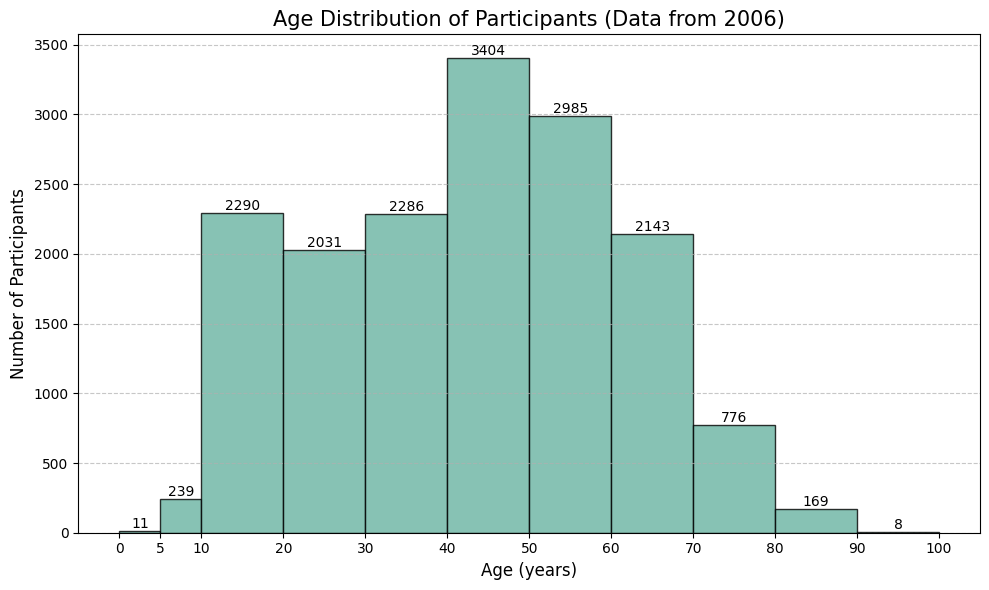
\includegraphics[width=0.72\textwidth]{age_dist.png}
\caption{Age distribution of participants.}
\label{fig:age_distribution}
\end{figure}

\subsection{Measured and Self Estimated Blood Pressure}

The dataset includes both measured and self estimated blood pressure. In Figure~\ref{fig:measured_estimated_bp}, density refers to the scaled height of the distribution, so that the total area under each curve equals one. This allows comparison of distributional shape even when groups differ in frequency.

The measured blood pressure distributions were wider than the self estimated distributions, especially for systolic blood pressure. This indicates that participants tended to report values concentrated around common reference points, while actual measurements showed greater variation.

\begin{figure}[!htbp]
\centering
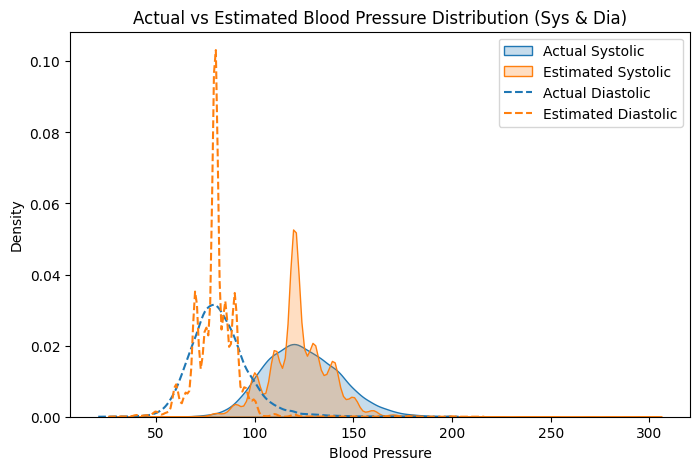
\includegraphics[width=0.72\textwidth]{sys_dia_comparison.png}
\caption{Distribution of measured and self estimated blood pressure values.}
\label{fig:measured_estimated_bp}
\end{figure}

\subsection{Group Differences and Correlations}

Male participants generally showed higher systolic and diastolic blood pressure values than female participants, although both groups had substantial internal variation.

\begin{figure}[!htbp]
\centering
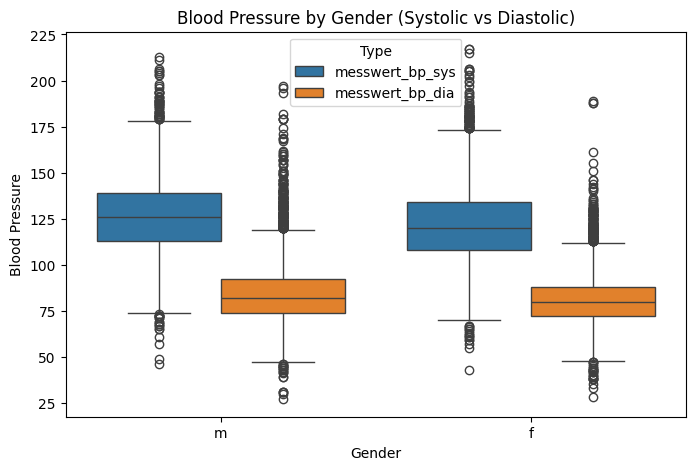
\includegraphics[width=0.70\textwidth]{gender_comparison.png}
\caption{Blood pressure distributions by gender.}
\label{fig:gender_bp}
\end{figure}

The correlation matrix showed a strong positive relationship between measured systolic and diastolic blood pressure. Age was moderately correlated with both outcomes. Estimated blood pressure values were also positively correlated with measured values, although the correlations were weaker than those between the measured blood pressure variables.

\begin{figure}[!htbp]
\centering
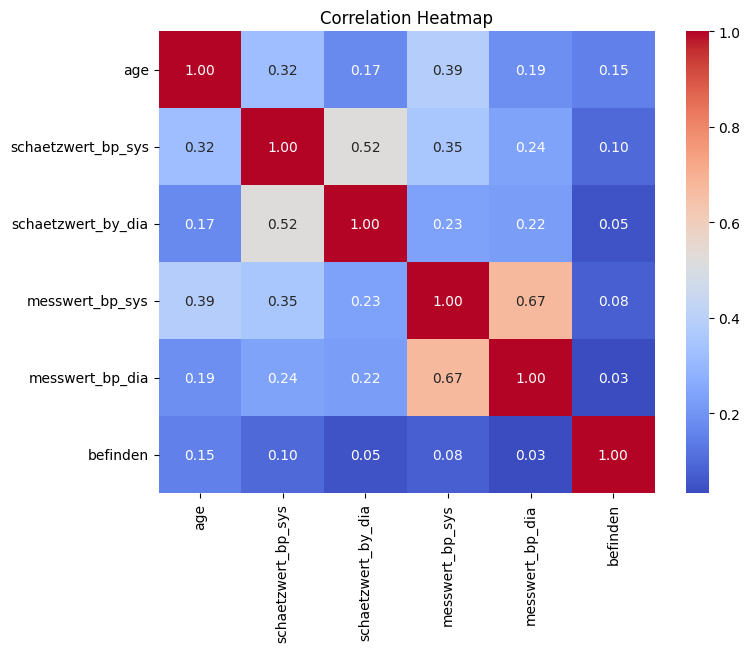
\includegraphics[width=0.72\textwidth]{correlation.png}
\caption{Correlation matrix of numerical variables.}
\label{fig:correlation}
\end{figure}

\subsection{Exploratory Findings}

The exploratory analysis suggested three patterns that guided the later modelling. First, age was strongly related to blood pressure and had to be treated as a central predictor. Second, measured and self estimated blood pressure differed substantially, indicating limited participant awareness of actual blood pressure values. Third, simple demographic variables explained only part of the observed variation, motivating both statistical modelling and machine learning approaches.
\section{Classical Statistical Modelling}

\subsection{Linear Regression Analysis}

To quantify the association between participant characteristics and blood pressure, separate Ordinary Least Squares (OLS) regression models were fitted for systolic and diastolic blood pressure.

The explanatory variables included age, sex, smoking status, known diabetes status, known cholesterol status, treatment status, and self reported health condition.

The general model specification was:

\[
BP_i = \beta_0 + \beta_1 Age_i + \beta_2 Sex_i + \beta_3 Smoking_i + \cdots + \varepsilon_i
\]

where \(BP_i\) represents the blood pressure value of participant \(i\), \(\beta_j\) are regression coefficients, and \(\varepsilon_i\) is the residual error term.

\subsection{Model Performance}

The systolic blood pressure model achieved an R\textsuperscript{2} of 0.155, while the diastolic model achieved an R\textsuperscript{2} of 0.040.

\begin{table}[H]
\centering
\caption{Summary of OLS model performance.}
\label{tab:ols_performance}
\begin{tabular}{lcc}
\toprule
Outcome & R\textsuperscript{2} & Adjusted R\textsuperscript{2} \\
\midrule
Systolic BP & 0.155 & 0.154 \\
Diastolic BP & 0.040 & 0.039 \\
\bottomrule
\end{tabular}
\end{table}

Although the explanatory power of the models was modest, the regression framework provides interpretable estimates that allow the relative importance of predictors to be assessed.

\subsection{Regression Results}

\begin{table}[H]
\centering
\caption{OLS coefficient estimates for systolic and diastolic blood pressure.}
\label{tab:ols_coefficients}
\small
\begin{tabular}{lcccc}
\toprule
Predictor & $\beta$ Systolic & p-value & $\beta$ Diastolic & p-value \\
\midrule
Age & +0.321 & $<0.001$ & +0.098 & $<0.001$ \\

Male Sex & +4.846 & $<0.001$ & +3.578 & $<0.001$ \\

Smoking & +0.211 & 0.599 & +0.801 & 0.011 \\

Known Blood Sugar & +1.400 & $<0.001$ & +0.560 & 0.089 \\

Known Cholesterol & -0.583 & 0.131 & +0.027 & 0.929 \\

Treatment Status & +8.221 & $<0.001$ & +2.483 & $<0.001$ \\

Wellbeing & +0.125 & 0.528 & -0.180 & 0.249 \\
\bottomrule
\end{tabular}
\end{table}
The regression results identified age, sex, and treatment status as the strongest predictors of blood pressure.
\subsection{Interpretation of Coefficients}

Age was one of the strongest predictors in both models. Each additional year of age was associated with an increase of approximately 0.32 mmHg in systolic blood pressure and 0.10 mmHg in diastolic blood pressure.

Male participants exhibited significantly higher blood pressure values than females after adjustment for the remaining variables. The estimated differences were approximately 4.8 mmHg for systolic blood pressure and 3.6 mmHg for diastolic blood pressure.

Treatment status showed the largest coefficient in both models. Participants receiving hypertension treatment exhibited substantially higher blood pressure values than untreated individuals. This finding is most plausibly explained by reverse causation, as treatment status serves as an indicator of existing hypertension rather than a causal determinant of elevated blood pressure.

Known diabetes status was positively associated with systolic blood pressure, whereas smoking showed a small positive association with diastolic blood pressure. In contrast, cholesterol awareness and self reported wellbeing were not significant predictors after adjustment for the remaining variables.

\subsection{Comparison with Random Forest Models}

The OLS and Random Forest approaches provide complementary perspectives on the dataset.

The Random Forest models achieved slightly higher predictive performance, particularly after incorporating temporal and environmental variables. In contrast, the OLS models provide interpretable estimates of effect size and direction.

Despite their methodological differences, both approaches identified age as the dominant predictor of blood pressure. Treatment status and sex also emerged as important variables in both modelling frameworks, increasing confidence in the consistency of the findings.

\subsection{Key Findings}

The regression analysis identified age, sex, and treatment status as the strongest determinants of blood pressure within the study population.

Although the models explained only a modest proportion of total variation, they provided clear evidence regarding the direction and relative magnitude of the observed associations. These results complement the machine learning findings and provide an interpretable framework for understanding blood pressure variation in the dataset.
\section{Machine Learning Models for Blood Pressure Prediction}

\subsection{Modelling Strategy}

Random Forest regression was used to evaluate how well blood pressure could be predicted from the available variables. Unlike linear regression, Random Forest models can capture nonlinear relationships and interactions without requiring a predefined functional form.

The analysis was conducted in three stages. The first model used only demographic and health related variables. Temporal information derived from measurement timestamps was then added, followed by environmental variables obtained from historical weather records.

Model performance was assessed using the coefficient of determination (R\textsuperscript{2}), Mean Absolute Error (MAE), and Root Mean Squared Error (RMSE).

\subsection{Baseline Model}

The baseline multi output Random Forest model used age, gender, smoking status, known diabetes status, known cholesterol status, treatment status, and self reported health condition.

\begin{table}[H]
\centering
\caption{Baseline Random Forest regression performance.}
\label{tab:rf_baseline}
\begin{tabular}{lccc}
\toprule
Outcome & R\textsuperscript{2} & MAE (mmHg) & RMSE (mmHg) \\
\midrule
Systolic BP & 0.130 & 14.14 & 18.14 \\
Diastolic BP & 0.042 & 10.50 & 14.20 \\
\bottomrule
\end{tabular}
\end{table}

The model explained a limited proportion of blood pressure variation, indicating that important determinants were not captured by the available variables.

\subsection{Predictor Importance}

Feature importance scores consistently identified age as the dominant predictor. Treatment status, gender, and self reported health condition provided additional information, while smoking, diabetes awareness, and cholesterol awareness contributed comparatively little.

\begin{figure}[H]
\centering
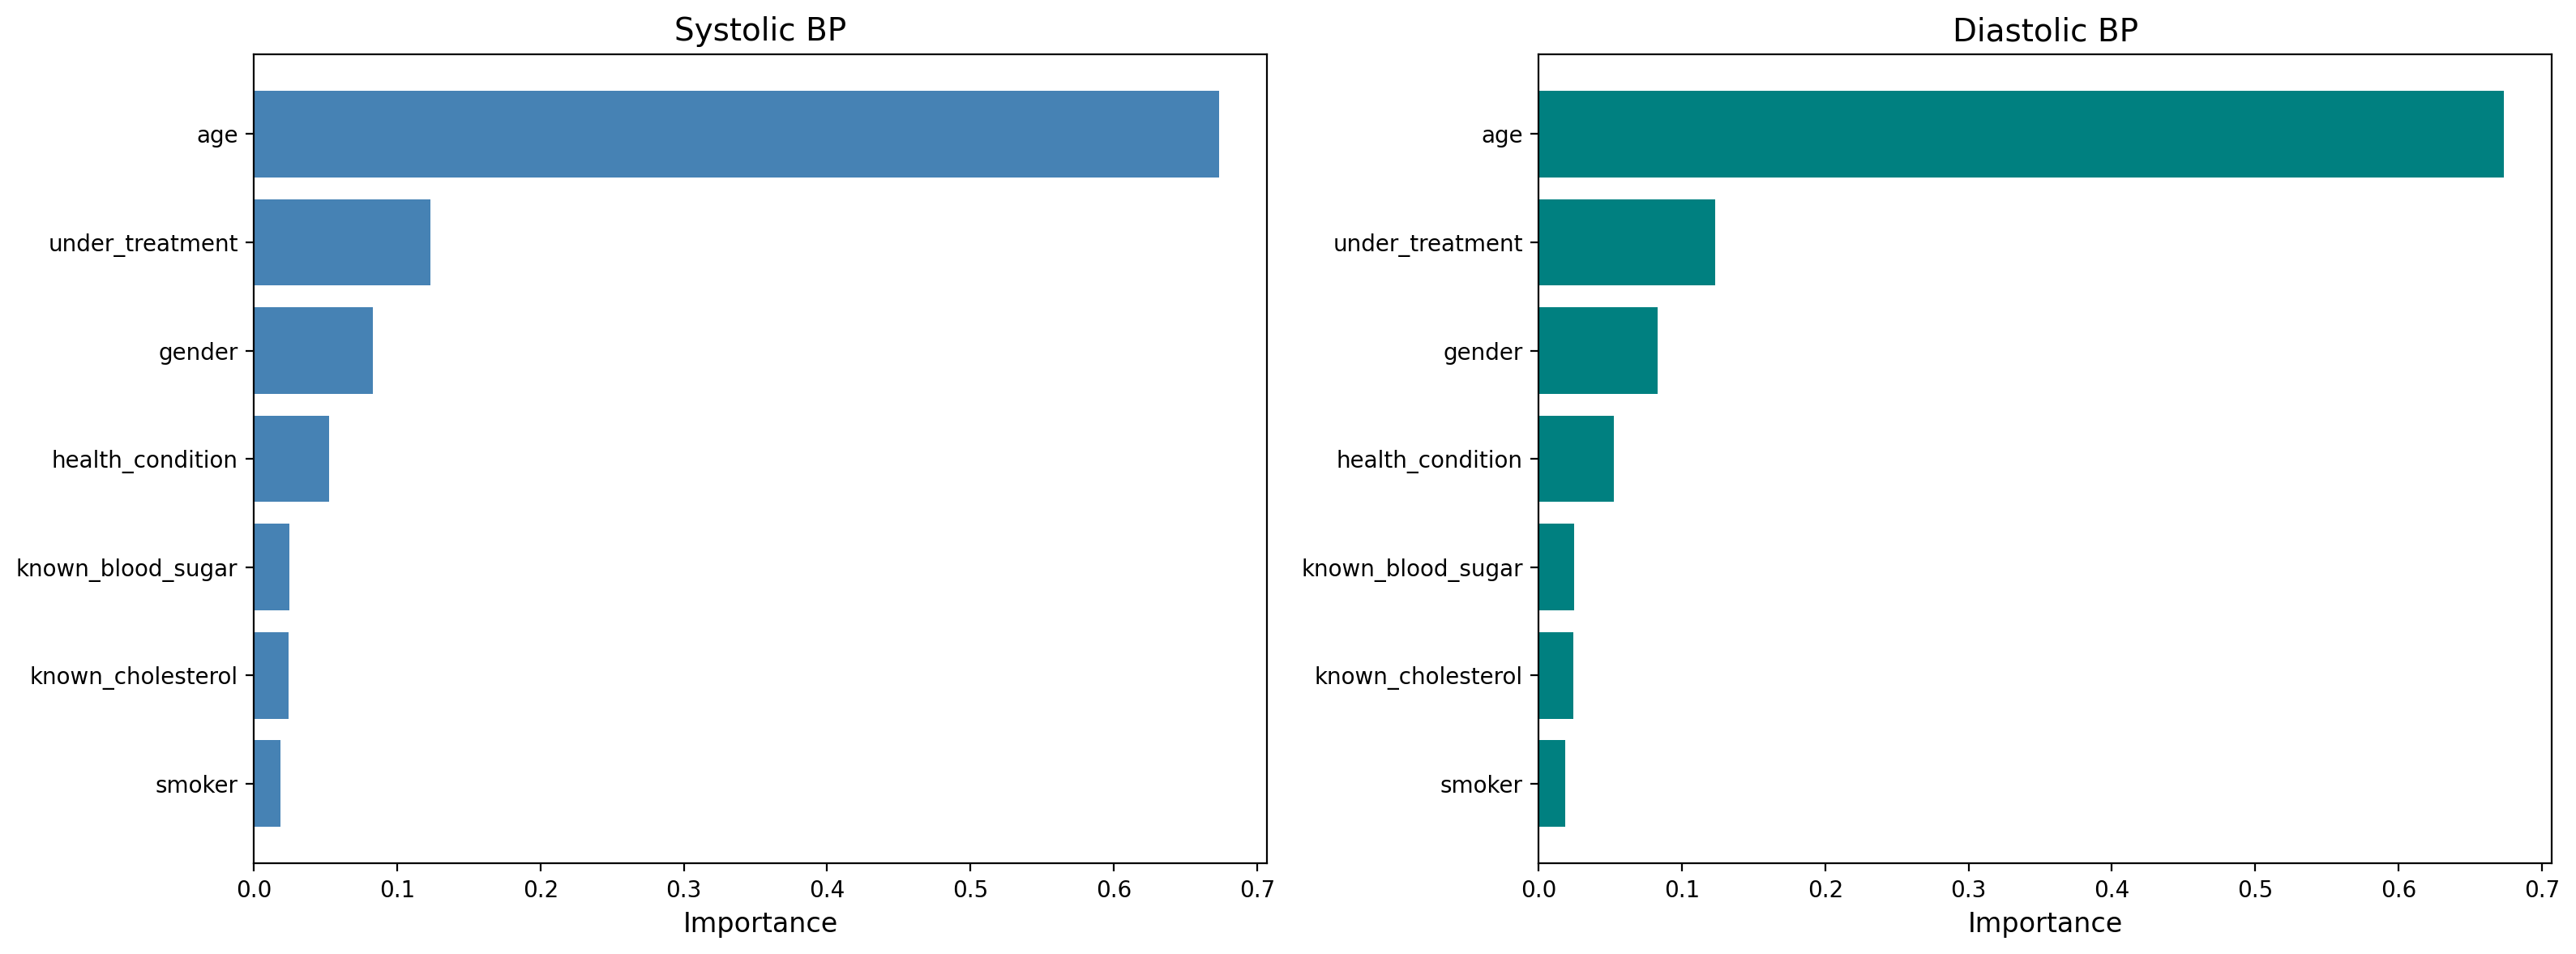
\includegraphics[width=0.95\textwidth]{bp_feature_importance_fig.png}
\caption{Random Forest feature importance rankings.}
\label{fig:rf_importance}
\end{figure}

The dominance of age is consistent with the exploratory analysis and later regression results.

\subsection{Model Validation}

To improve robustness, the train and test split was stratified by age group. Five fold cross validation was then applied to evaluate model stability.

Tree depth was varied to investigate the relationship between model complexity and predictive performance.

\begin{table}[H]
\centering
\caption{Cross validated performance across different tree depths.}
\label{tab:rf_depth}
\begin{tabular}{lc}
\toprule
Maximum Depth & Mean Cross Validated R\textsuperscript{2} \\
\midrule
3 & 0.138 \\
5 & 0.157 \\
10 & 0.163 \\
20 & 0.140 \\
Unlimited & 0.140 \\
\bottomrule
\end{tabular}
\end{table}

Performance improved with increasing tree depth up to approximately ten levels, after which performance declined. This behaviour suggests overfitting in more complex models.

\subsection{Temporal and Environmental Information}

Blood pressure varies throughout the day and may also be influenced by environmental conditions. Temporal variables included hour of day, day of week, month, and season. Environmental variables consisted of temperature and relative humidity obtained from historical weather records.

Adding temporal information improved model performance for both outcomes.

\begin{table}[H]
\centering
\caption{Performance improvement after adding temporal variables.}
\label{tab:temporal_results}
\begin{tabular}{lcc}
\toprule
Outcome & Baseline R\textsuperscript{2} & Temporal R\textsuperscript{2} \\
\midrule
Systolic BP & 0.130 & 0.176 \\
Diastolic BP & 0.042 & 0.086 \\
\bottomrule
\end{tabular}
\end{table}

The addition of weather variables resulted in further improvements.

\begin{table}[H]
\centering
\caption{Performance improvement after adding weather variables.}
\label{tab:weather_results}
\begin{tabular}{lcc}
\toprule
Outcome & Temporal R\textsuperscript{2} & Weather R\textsuperscript{2} \\
\midrule
Systolic BP & 0.176 & 0.192 \\
Diastolic BP & 0.086 & 0.097 \\
\bottomrule
\end{tabular}
\end{table}

\begin{table}[H]
\centering
\caption{Mean absolute error across model versions.}
\label{tab:mae_results}
\begin{tabular}{lcc}
\toprule
Model & Systolic MAE & Diastolic MAE \\
\midrule
Baseline RF & 14.14 & 10.50 \\
Temporal RF & 13.81 & 10.19 \\
Weather RF & 13.60 & 10.05 \\
\bottomrule
\end{tabular}
\end{table}

Although the improvements were modest, they occurred consistently across both outcomes.

\subsection{Environmental Effects}

The weather enhanced model suggested a weak inverse relationship between temperature and predicted blood pressure.

\begin{figure}[H]
\centering
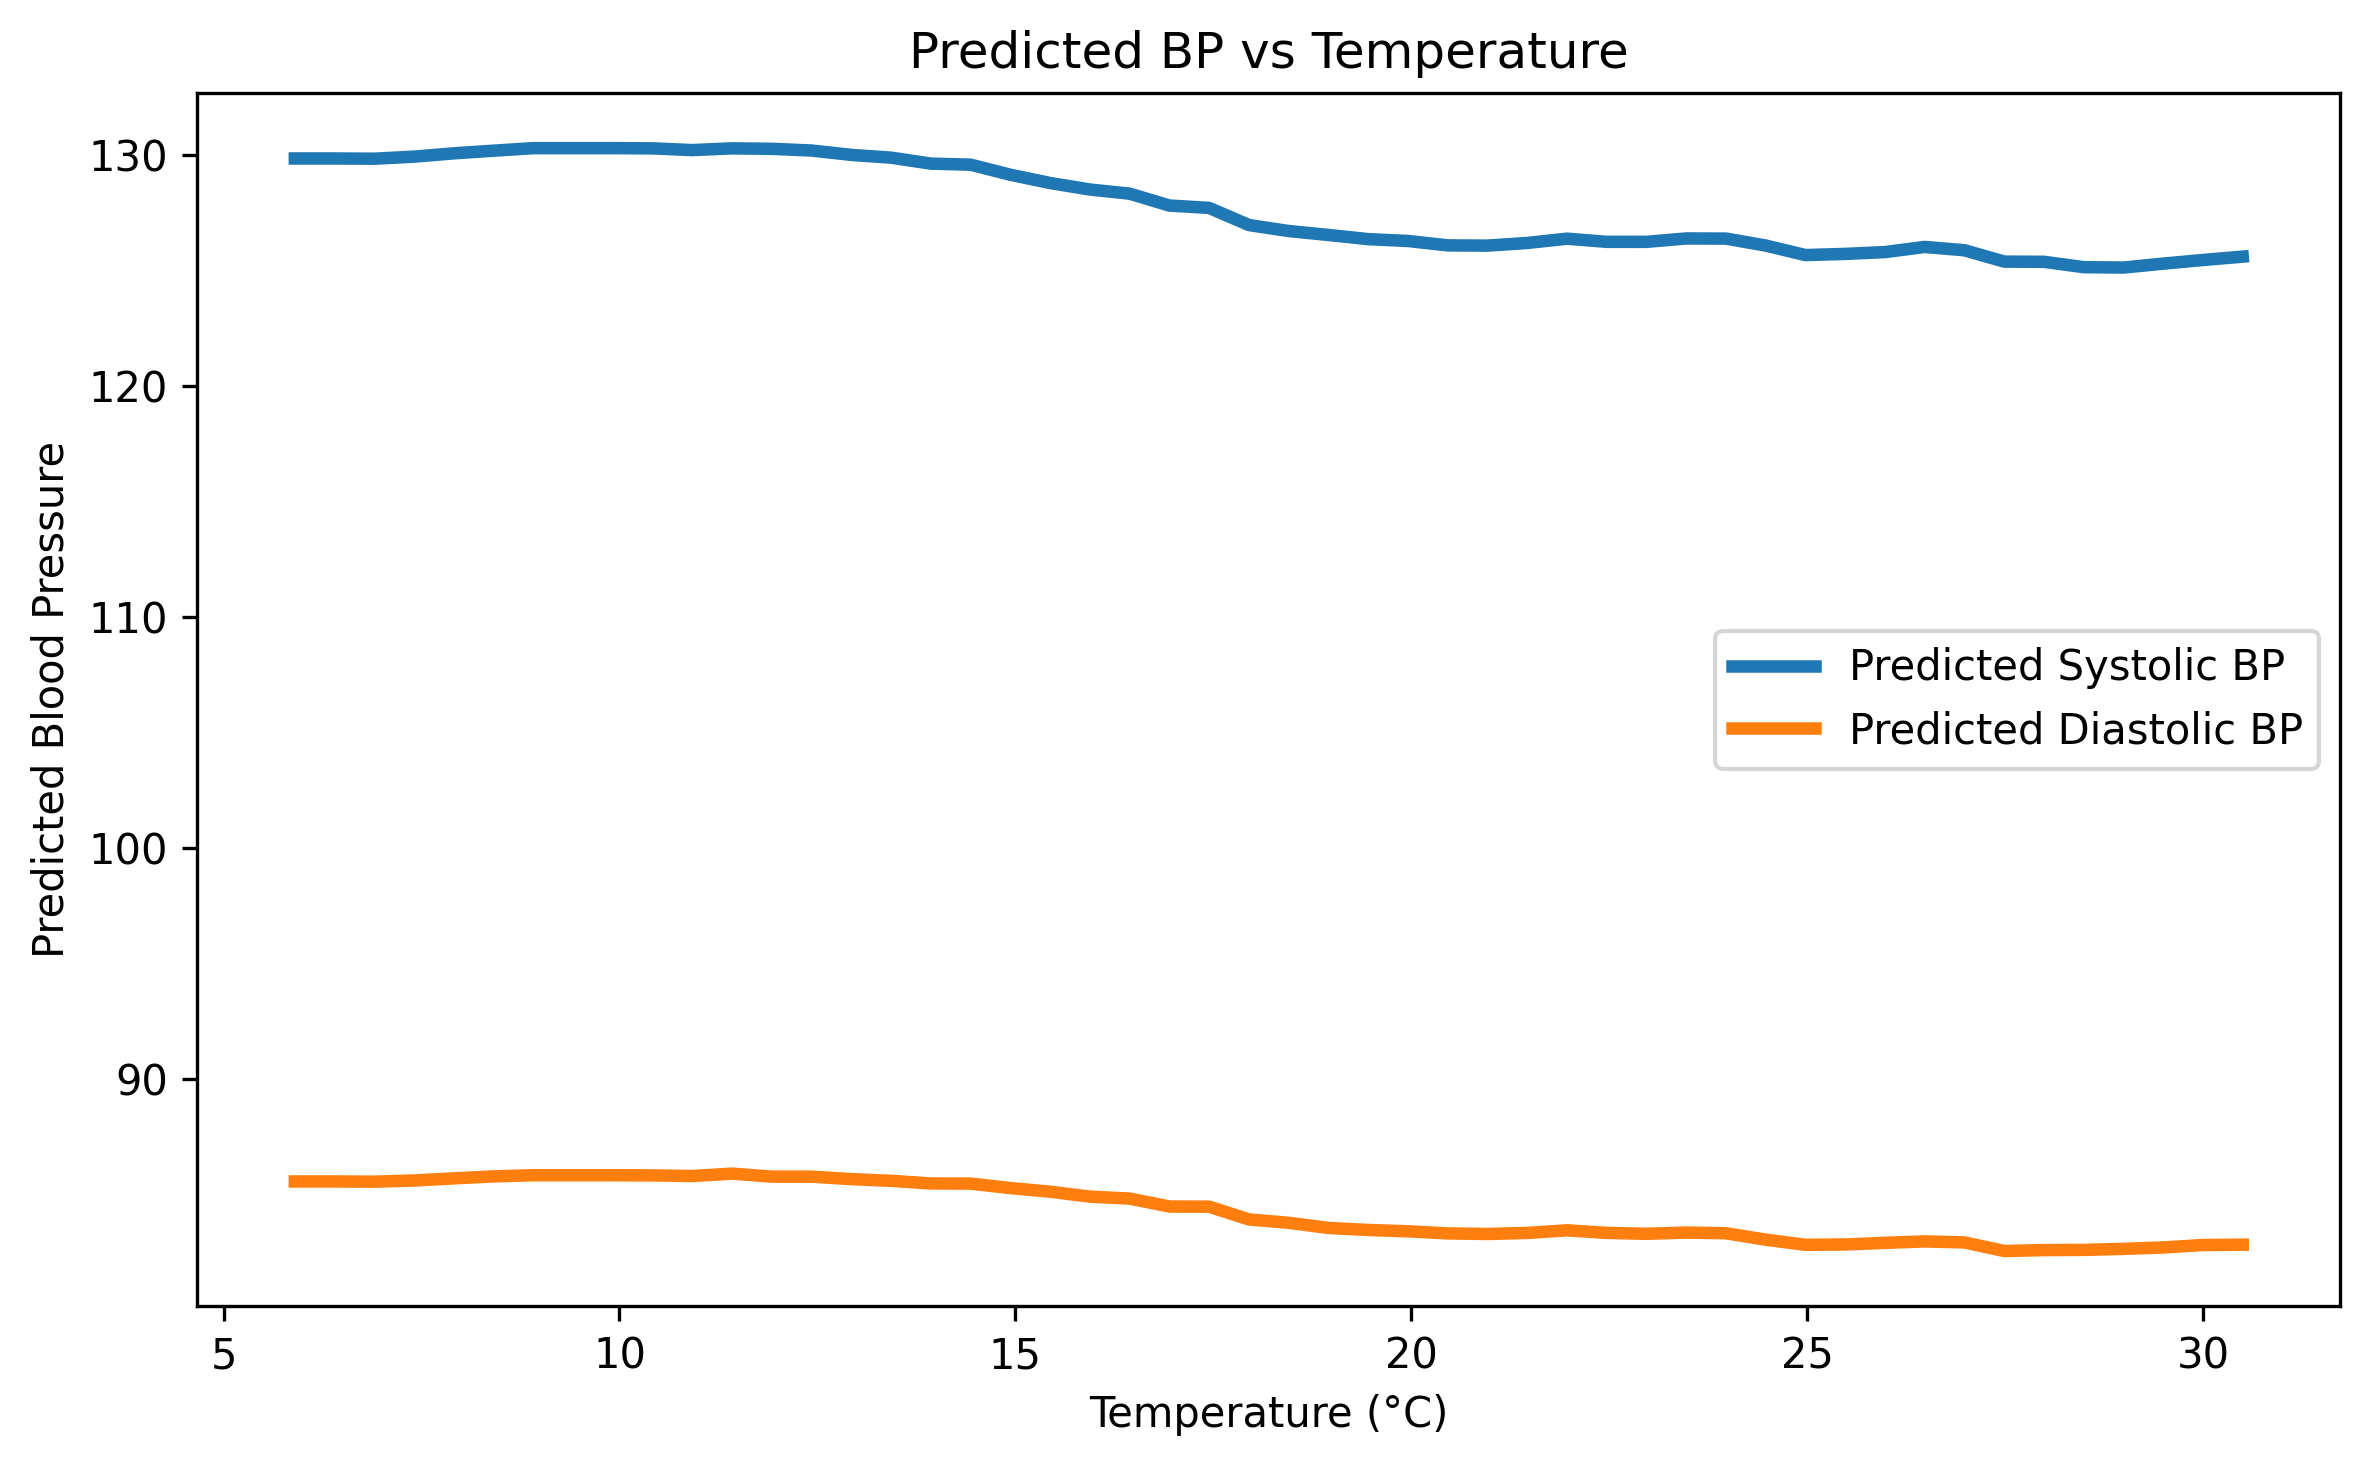
\includegraphics[width=0.72\textwidth]{predicted_bp_vs_temperature.png}
\caption{Predicted blood pressure as a function of temperature.}
\label{fig:temperature_effect}
\end{figure}

Residual diagnostics did not indicate substantial temperature related bias.

\begin{figure}[htbp]
\centering
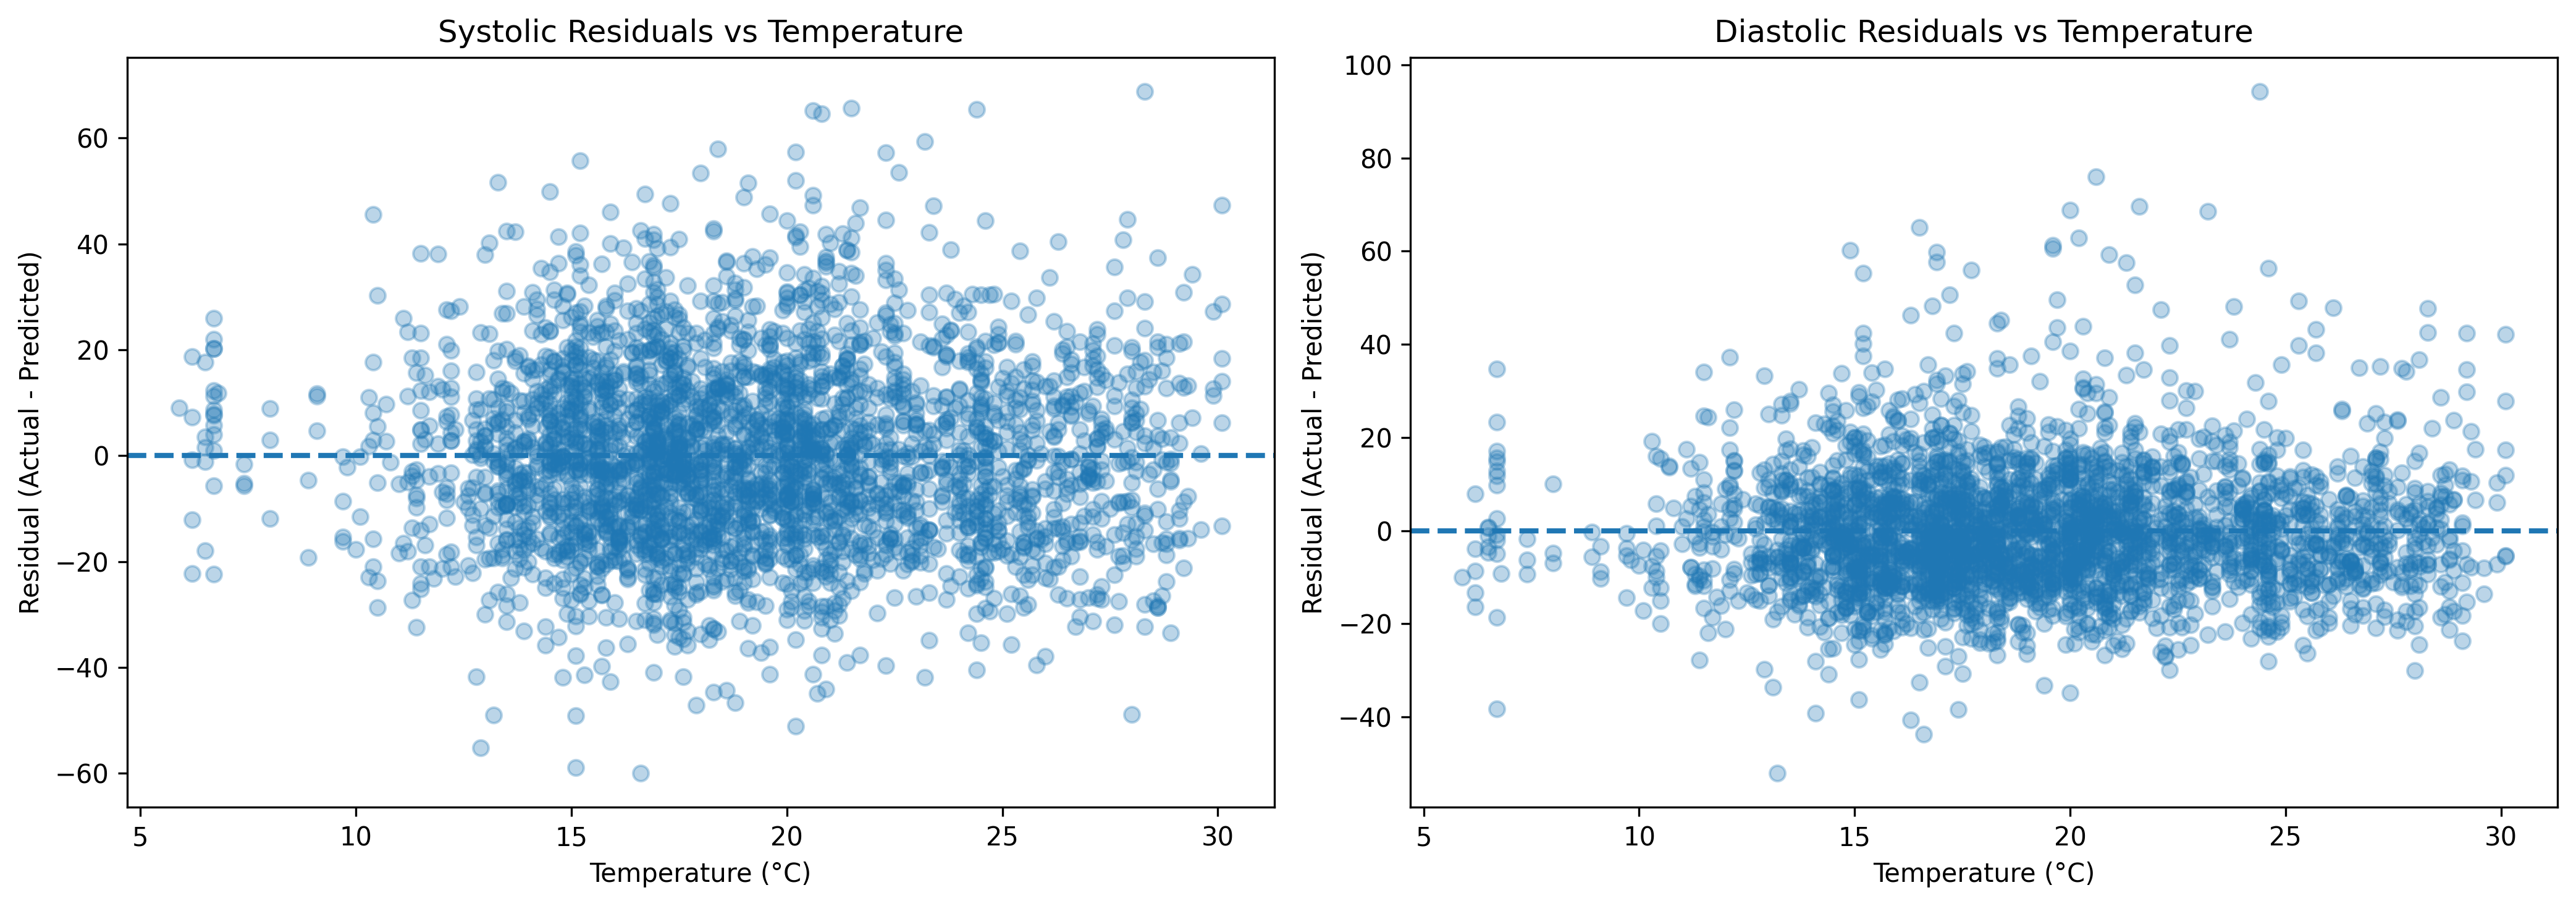
\includegraphics[width=0.72\textwidth]{residuals_vs_temperature.png}
\caption{Residual diagnostics for the weather enhanced Random Forest model.}
\label{fig:residuals}
\end{figure}

\subsection{Key Findings}

Three conclusions emerge from the Random Forest analysis. First, age is by far the most influential predictor of blood pressure. Second, temporal and environmental information improve predictive performance, although the gains are modest. Third, even the best performing model explains less than 20\% of the variation in systolic blood pressure, indicating that important determinants were not available in the dataset.
\section{Classification of Elevated Blood Pressure}

\subsection{Classification Framework}

In addition to predicting exact blood pressure values, a classification approach was used to identify participants with elevated blood pressure. This task is more closely aligned with clinical screening, where the primary objective is to determine whether a patient exceeds a diagnostic threshold.

Two binary classification problems were considered:

\[
\text{Systolic Blood Pressure} \geq 140 \text{ mmHg}
\]

\[
\text{Diastolic Blood Pressure} \geq 90 \text{ mmHg}
\]

Because elevated blood pressure cases were less frequent than normal cases, weighted Random Forest classifiers were used to address class imbalance.

Performance was evaluated using accuracy, precision, recall, and F1 score.

\subsection{Classification Performance}

Table~\ref{tab:classification_sys} summarises the results for systolic blood pressure classification.

\begin{table}[H]
\centering
\caption{Classification performance for elevated systolic blood pressure.}
\label{tab:classification_sys}
\begin{tabular}{lc}
\toprule
Metric & Value \\
\midrule
Accuracy & 0.712 \\
Precision & 0.394 \\
Recall & 0.560 \\
F1 Score & 0.463 \\
\bottomrule
\end{tabular}
\end{table}

Table~\ref{tab:classification_dia} presents the corresponding results for diastolic blood pressure.

\begin{table}[H]
\centering
\caption{Classification performance for elevated diastolic blood pressure.}
\label{tab:classification_dia}
\begin{tabular}{lc}
\toprule
Metric & Value \\
\midrule
Accuracy & 0.640 \\
Precision & 0.367 \\
Recall & 0.519 \\
F1 Score & 0.430 \\
\bottomrule
\end{tabular}
\end{table}

Classification performance was consistently stronger for systolic blood pressure. In both models, more than half of elevated blood pressure cases were correctly identified.

\begin{figure}[H]
\centering
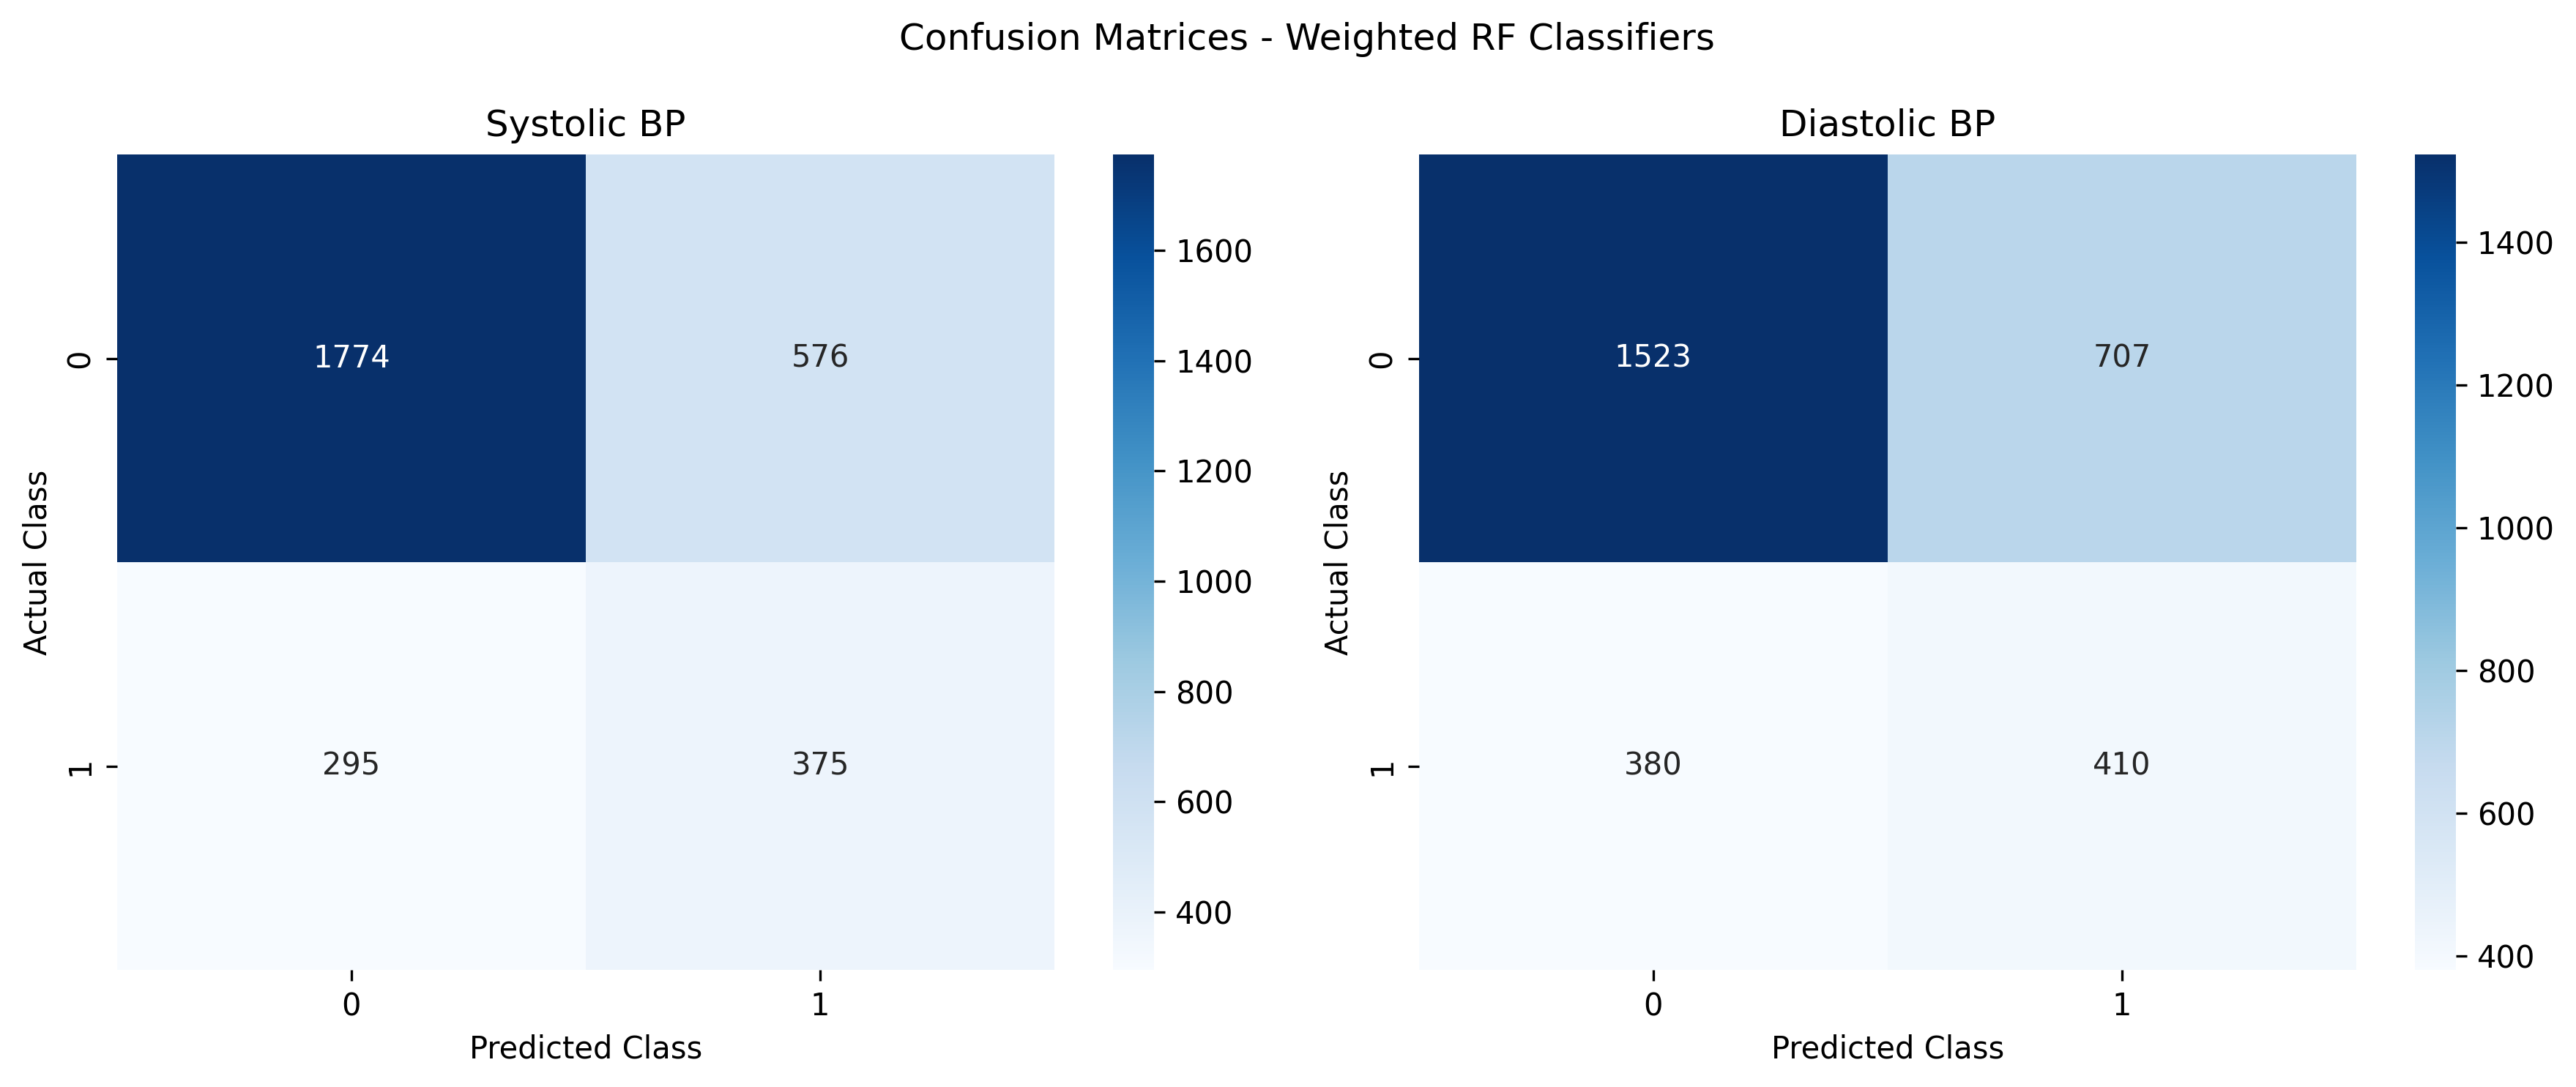
\includegraphics[width=0.78\textwidth]{classification_confusion_matrices.png}
\caption{Confusion matrices for systolic and diastolic blood pressure classification.}
\label{fig:confusion_matrices}
\end{figure}

\subsection{Threshold Sensitivity}

The influence of alternative classification thresholds was evaluated using a sensitivity analysis.

\begin{figure}[H]
\centering
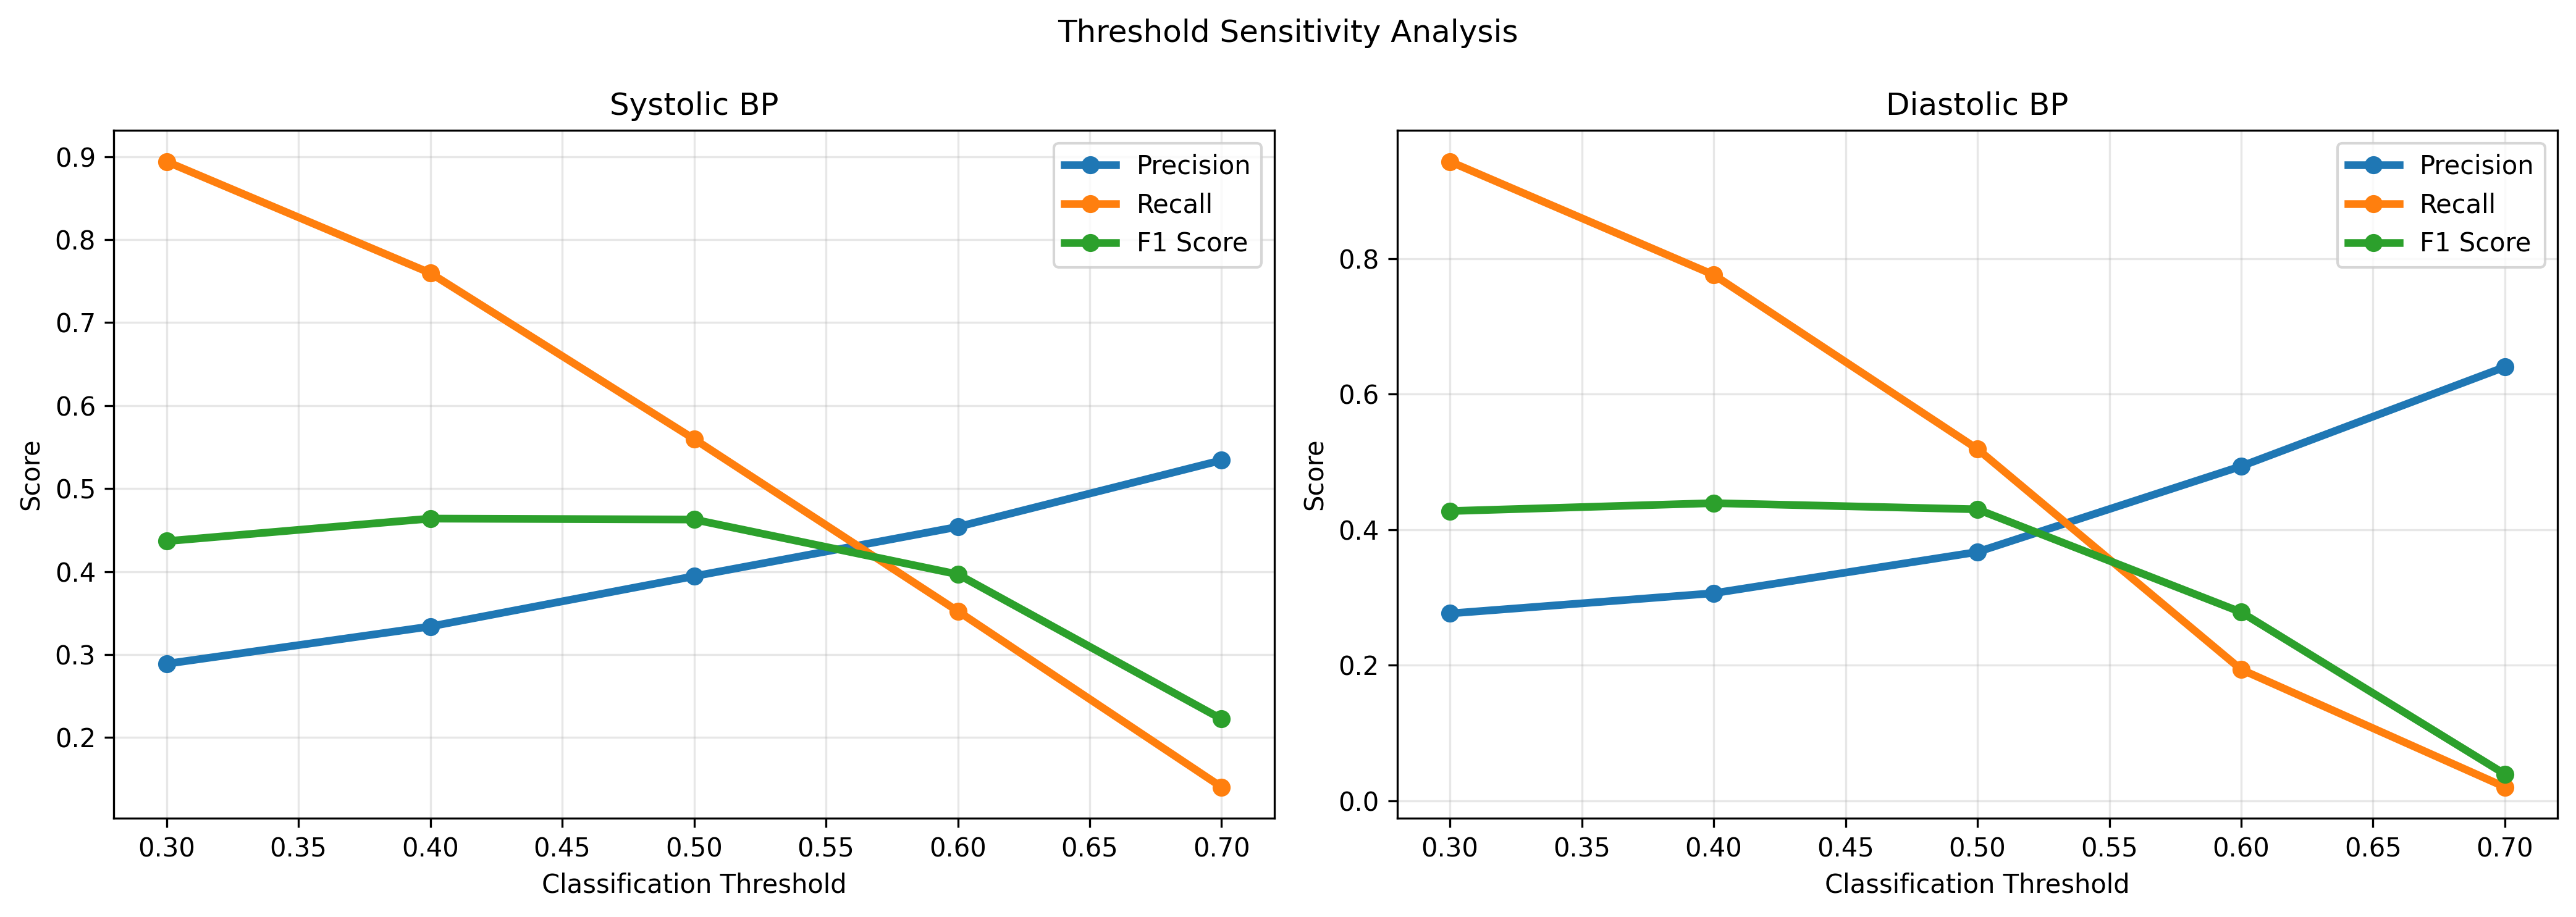
\includegraphics[width=0.78\textwidth]{threshold_sensitivity.png}
\caption{Classification performance under different threshold values.}
\label{fig:threshold_analysis}
\end{figure}

Lower thresholds increased recall and identified a larger number of potential cases, whereas higher thresholds improved precision and reduced false positives. This behaviour reflects the expected trade off between sensitivity and specificity in medical screening applications.

\subsection{Key Findings}

The classification models performed better at identifying elevated blood pressure categories than predicting exact blood pressure values. Systolic classification achieved the strongest results, while diastolic classification remained moderately successful.

The results suggest that the available demographic and health related variables contain useful information for identifying individuals at increased risk. However, the modest precision values indicate that additional clinical variables would be required for reliable clinical decision support.
\section{Spatial and Socioeconomic Analysis}

\subsection{Rationale}

Blood pressure is influenced by individual level characteristics, but geographic context may also contribute to variation through differences in demographics, healthcare access, environmental conditions, and socioeconomic factors. To investigate these effects, spatial analyses were conducted at both district and NUTS3 levels.

The analysis focused on three questions:

\begin{enumerate}
\item Does blood pressure vary across urban and rural regions?
\item Is there evidence of spatial clustering?
\item Are socioeconomic indicators associated with blood pressure outcomes?
\end{enumerate}

\subsection{Urban Rural Patterns}

Municipalities were linked to the Eurostat urban rural typology and aggregated to the district level. Hypertension prevalence, mean systolic blood pressure, and mean diastolic blood pressure were compared across urban, intermediate, peri urban, rural, and remote rural districts.

\clearpage

\begin{figure}[!htbp]
\centering
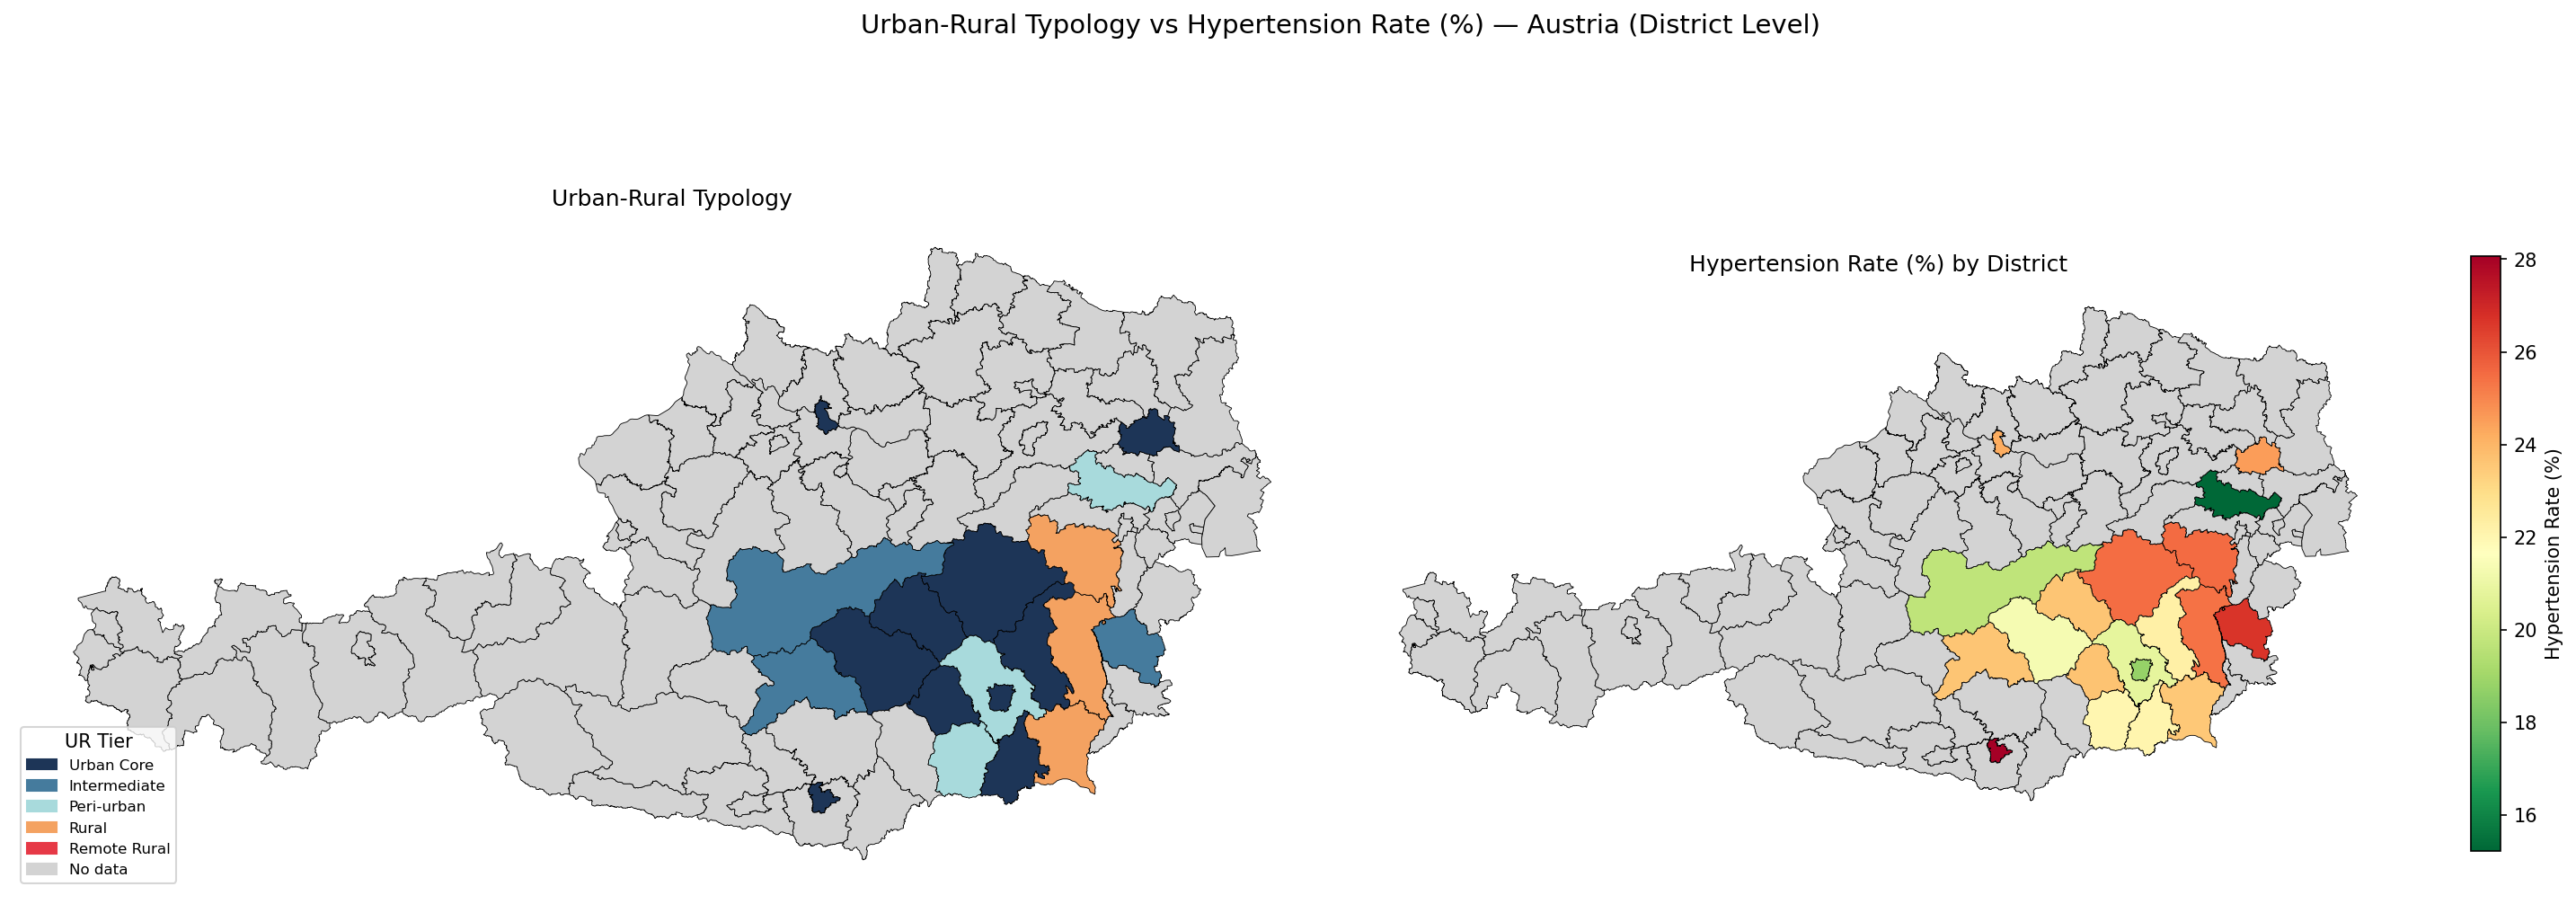
\includegraphics[width=0.82\textwidth]{map_ur_vs_hyp_district.png}
\caption{Urban rural typology and hypertension prevalence at district level.}
\label{fig:ur_hyp}
\end{figure}

\begin{figure}[!htbp]
\centering
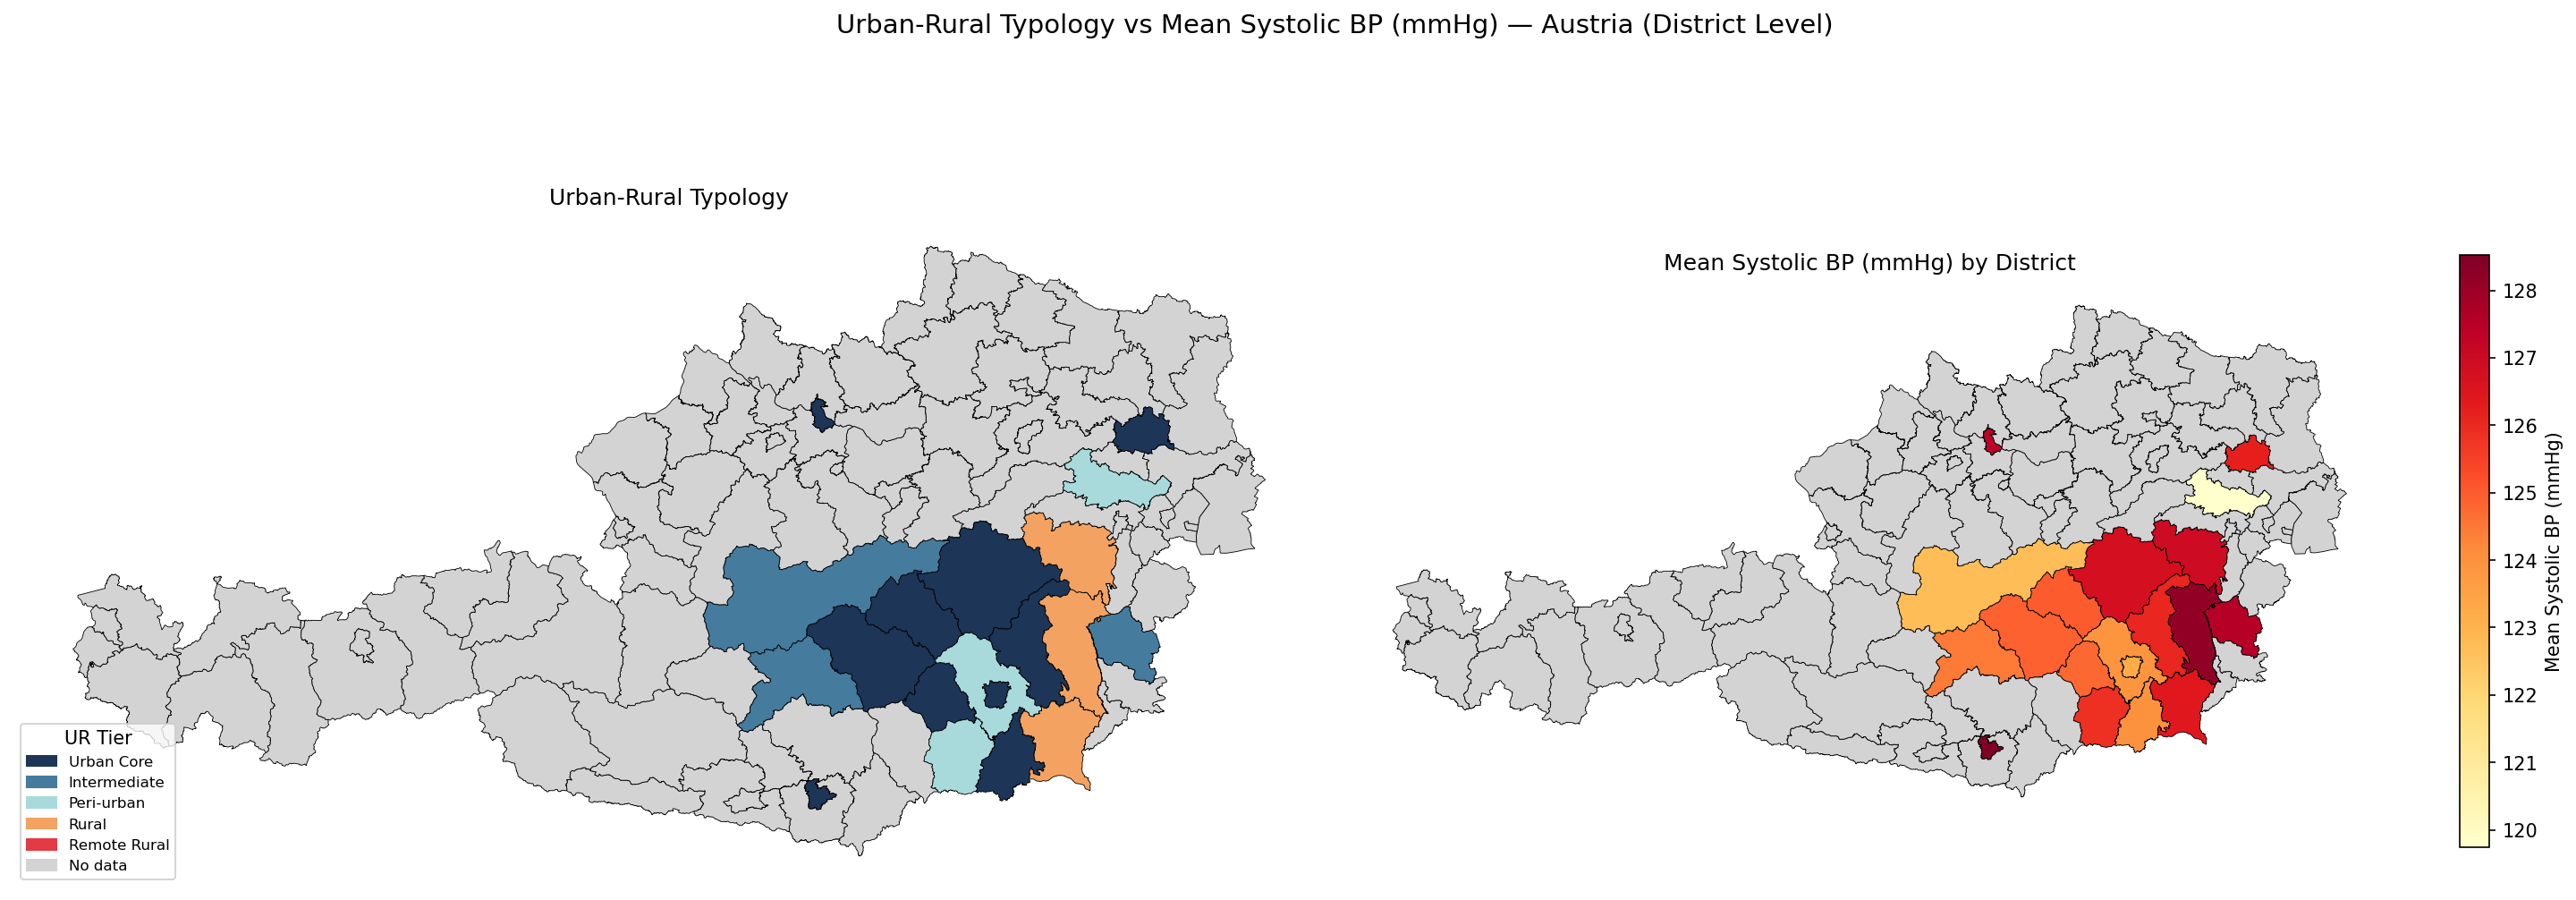
\includegraphics[width=0.82\textwidth]{map_ur_vs_sysbp_district.png}
\caption{Urban rural typology and mean systolic blood pressure at district level.}
\label{fig:ur_sysbp}
\end{figure}

\begin{figure}[!htbp]
\centering
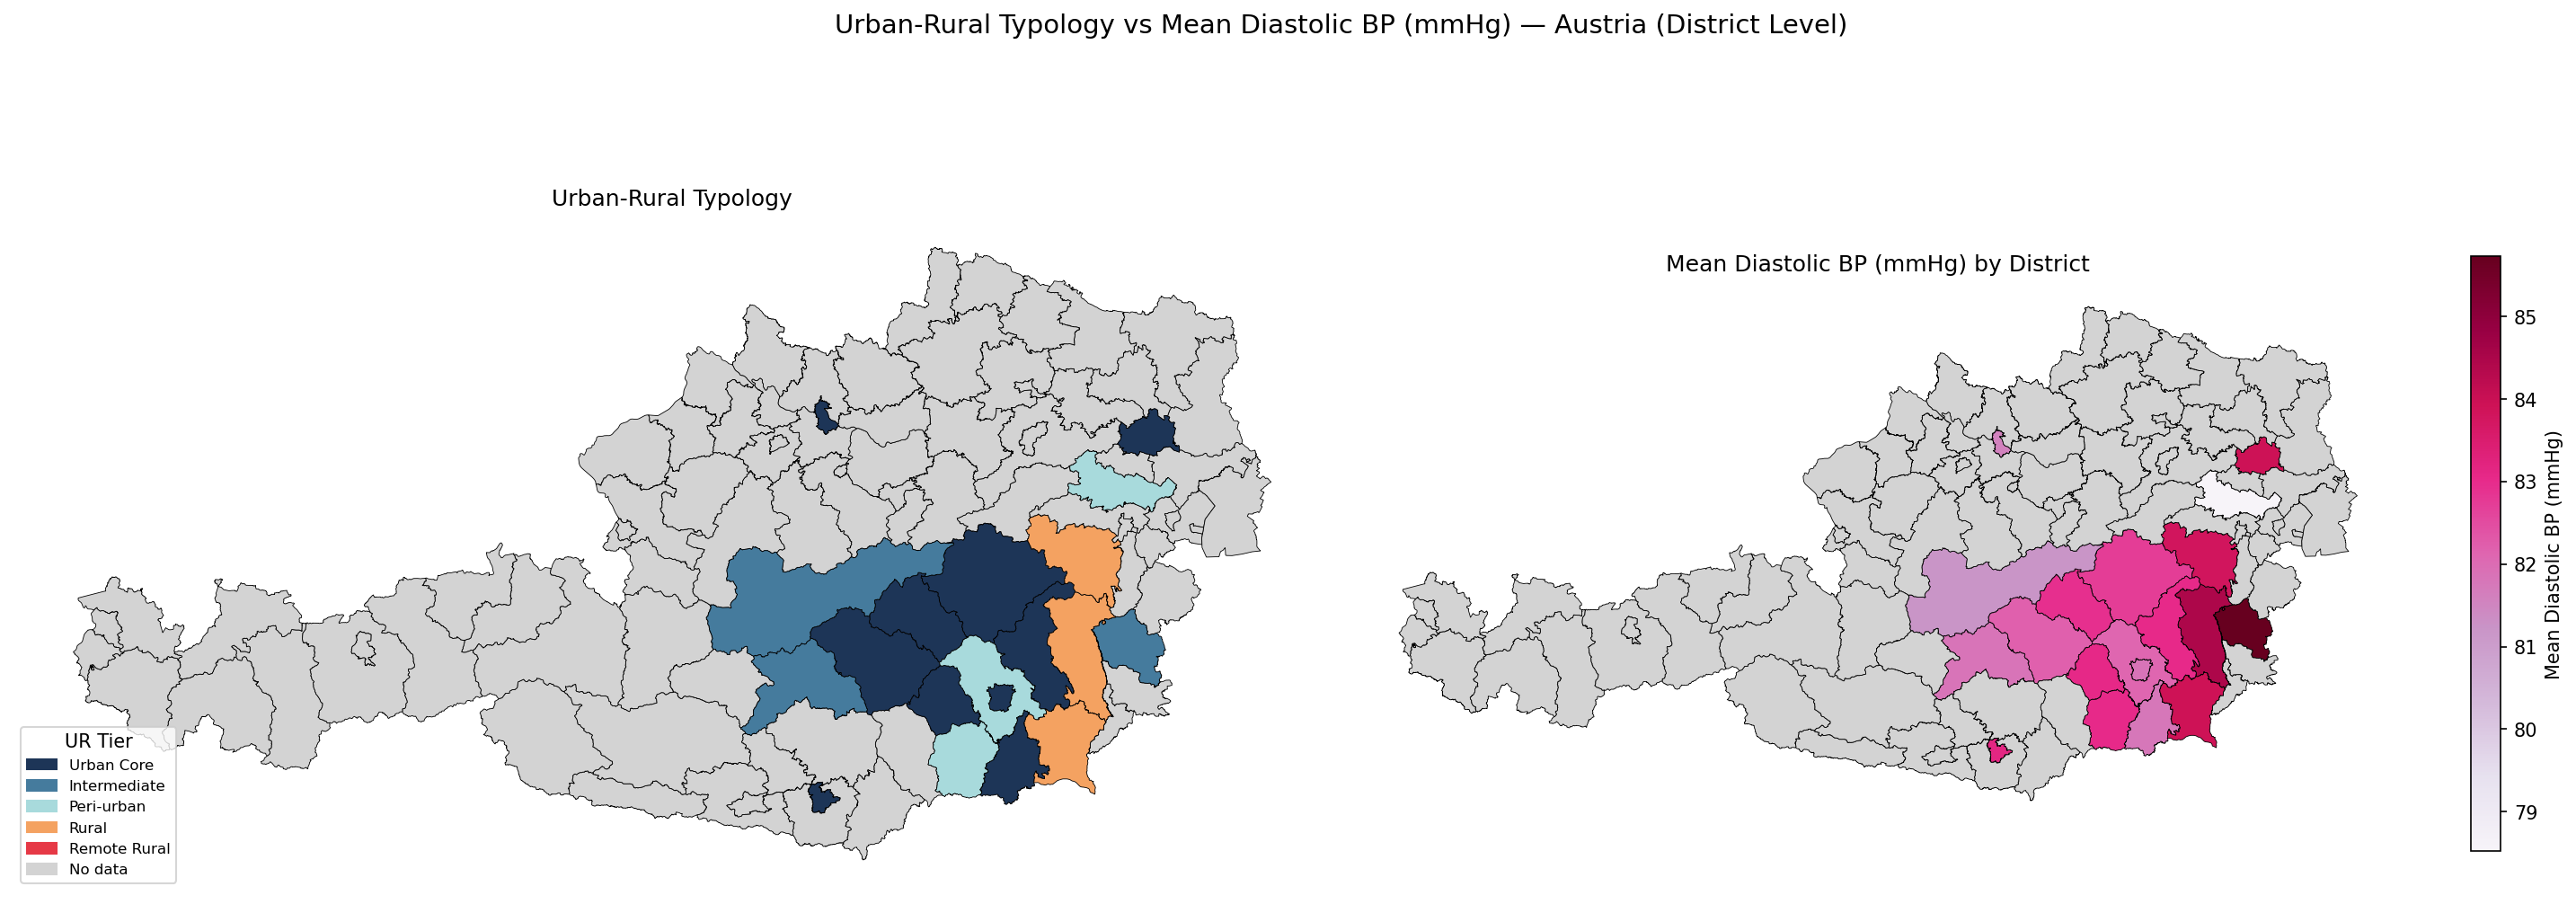
\includegraphics[width=0.82\textwidth]{map_ur_vs_diabp_district.png}
\caption{Urban rural typology and mean diastolic blood pressure at district level.}
\label{fig:ur_diabp}
\end{figure}

Although differences were observed between districts, no consistent gradient emerged across urbanisation categories. Elevated blood pressure and hypertension prevalence occurred in both urban and rural regions, suggesting that urbanisation alone does not explain geographic variation in cardiovascular risk.

\subsection{Spatial Clustering}

Spatial autocorrelation was assessed using Moran's I and Local Indicators of Spatial Association (LISA).

\begin{figure}[H]
\centering
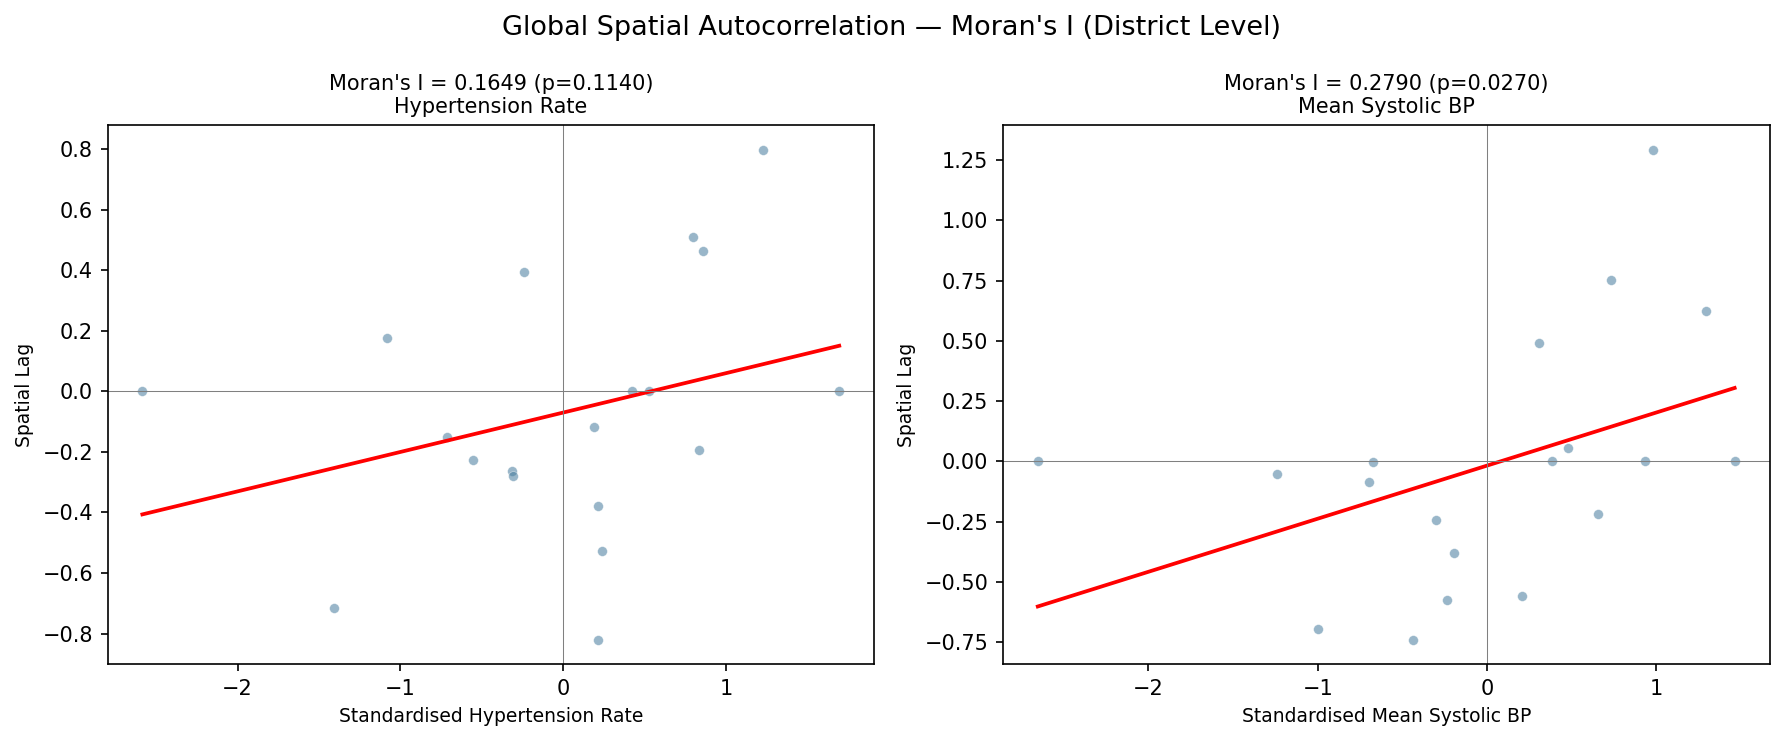
\includegraphics[width=0.75\textwidth]{morans_I_district.png}
\caption{Moran's I analysis at district level.}
\label{fig:morans_district}
\end{figure}

Positive spatial dependence was observed at the district level, indicating that neighbouring districts tended to exhibit similar blood pressure profiles.

To identify specific clusters and spatial outliers, LISA statistics were calculated.

\begin{figure}[H]
\centering
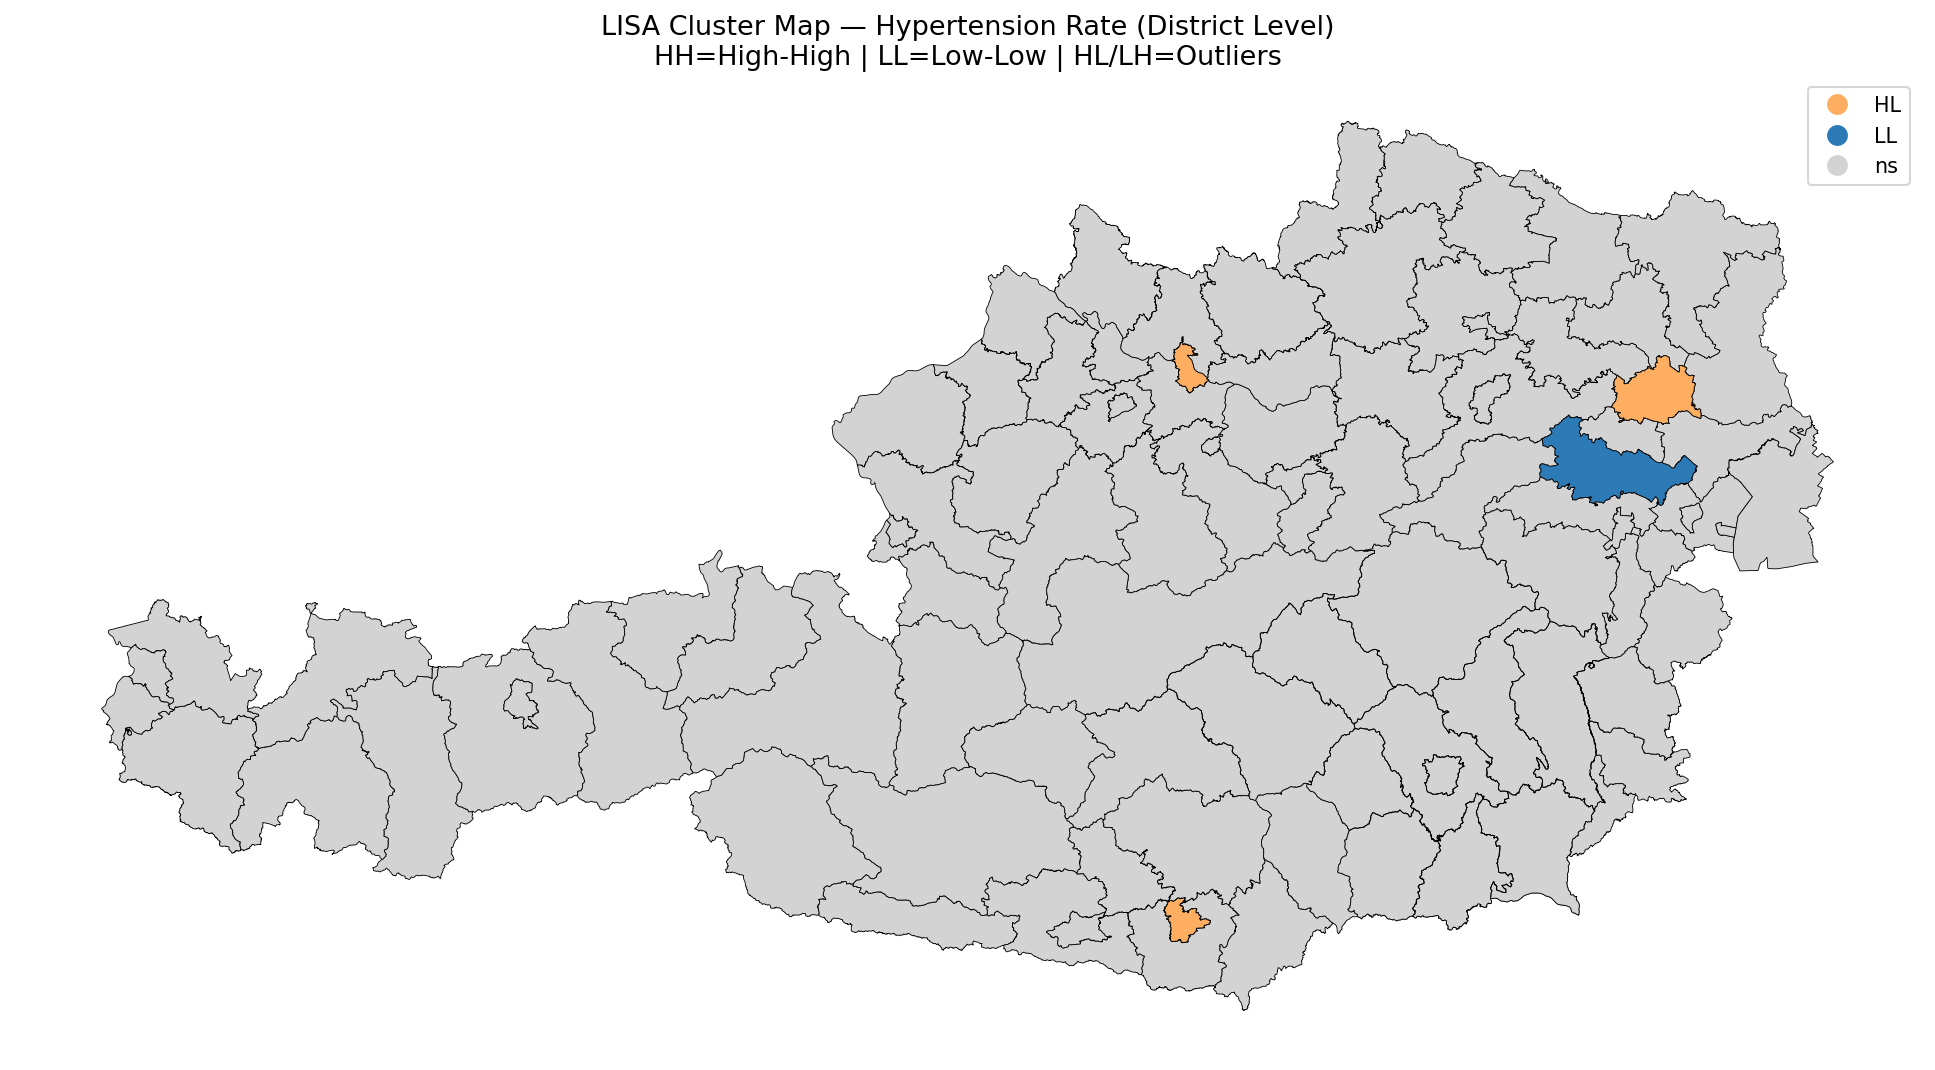
\includegraphics[width=0.49\textwidth]{lisa_clusters_hyp_district.png}
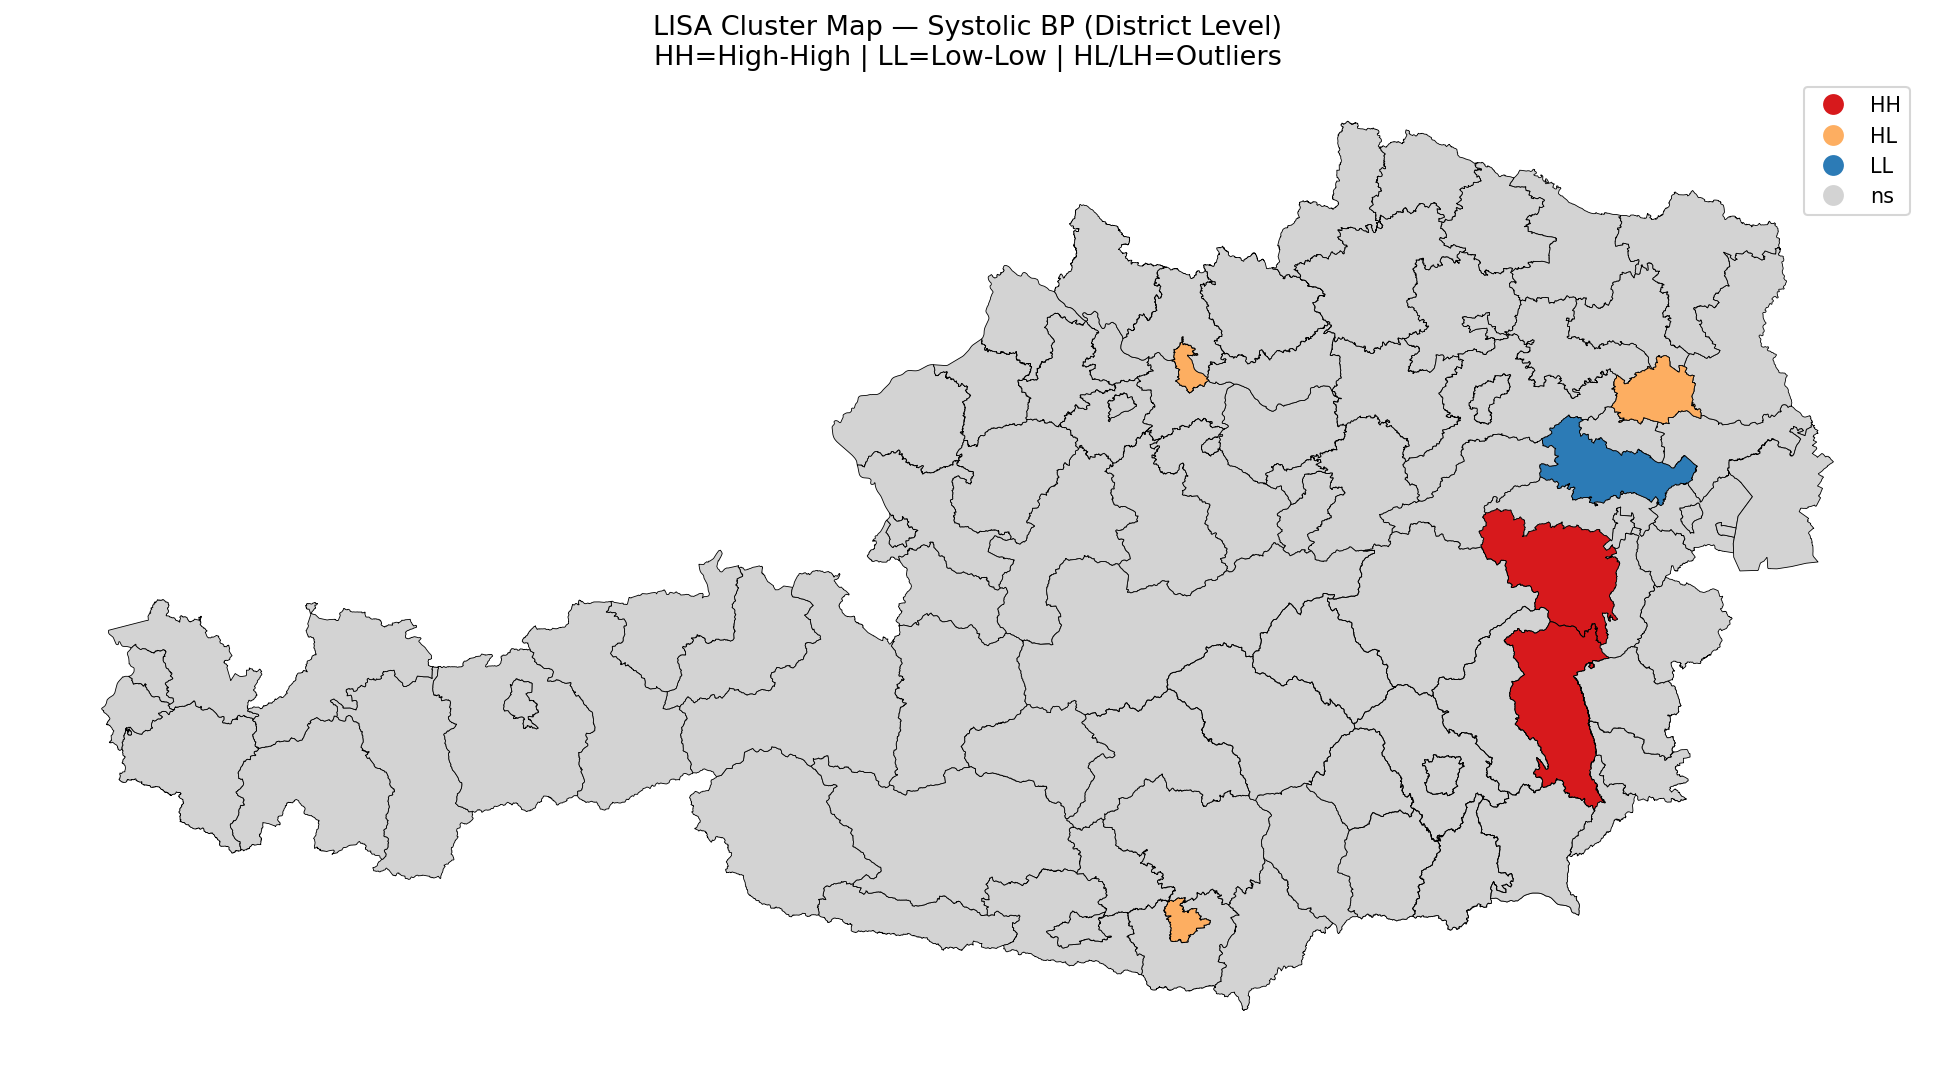
\includegraphics[width=0.49\textwidth]{lisa_clusters_sysbp_district.png}
\caption{LISA cluster maps for hypertension prevalence and mean systolic blood pressure at district level.}
\label{fig:lisa_district}
\end{figure}

Several notable patterns emerged. Baden formed a Low Low cluster characterised by consistently low hypertension prevalence and blood pressure values. Vienna, Linz, and Klagenfurt appeared as High Low outliers, while Hartberg Fürstenfeld and Neunkirchen formed a High High cluster with elevated systolic blood pressure values.

These findings indicate that cardiovascular risk exhibits meaningful geographic structure rather than being randomly distributed across Austria.

\subsection{Regional Economic Indicators}

Regional GDP per capita was linked to NUTS3 regions to investigate whether economically stronger regions exhibited lower blood pressure levels.

\begin{figure}[H]
\centering
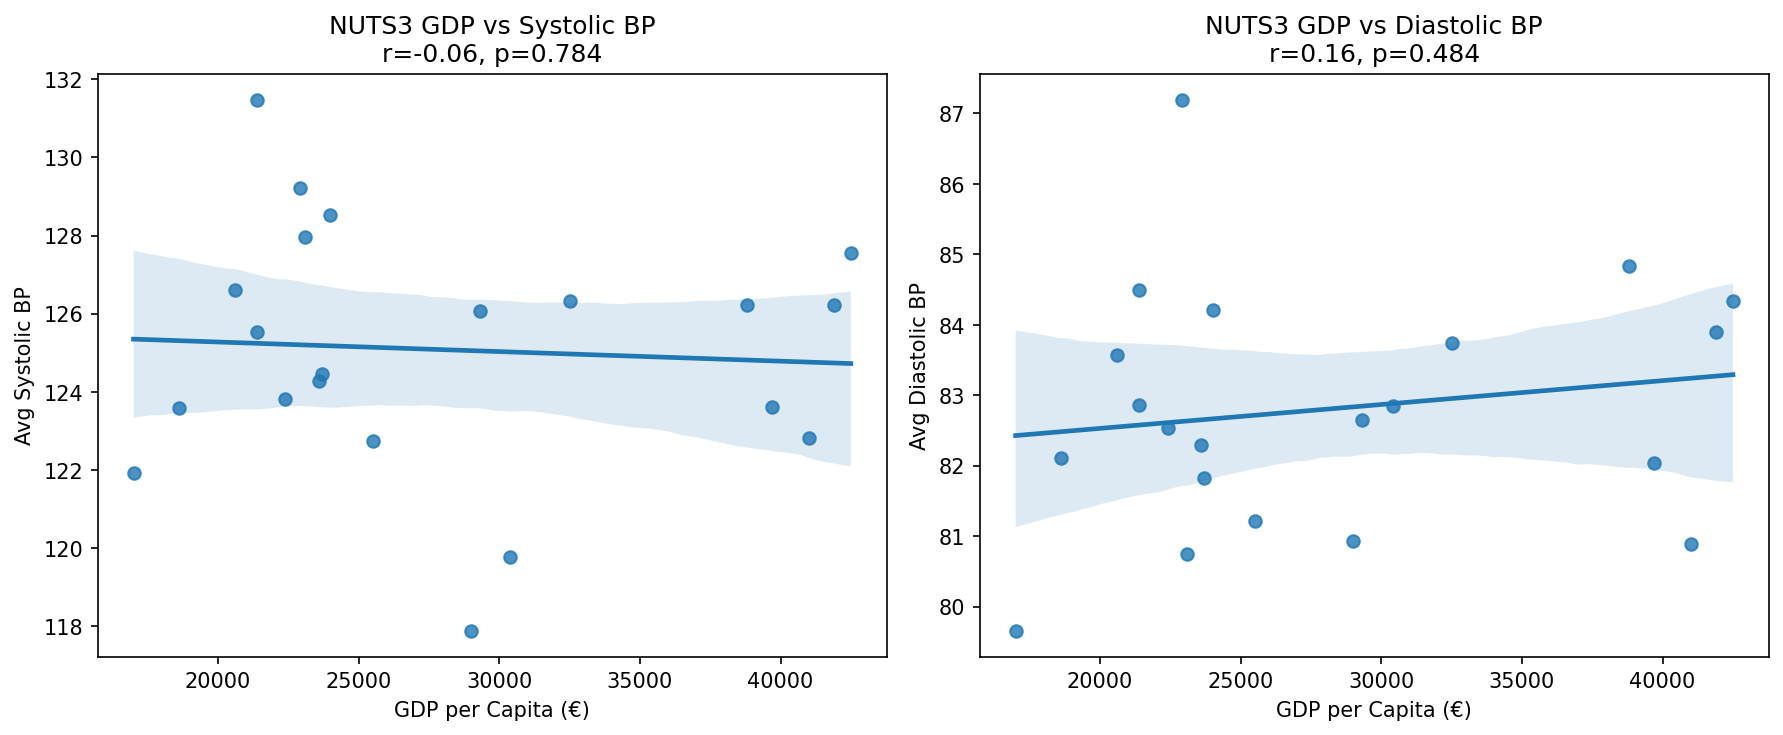
\includegraphics[width=0.80\textwidth]{nuts3_gdp_vs_bp.png}
\caption{Relationship between GDP per capita and blood pressure at the NUTS3 level.}
\label{fig:gdp_bp}
\end{figure}

Only a weak negative correlation was observed between GDP and systolic blood pressure ($r=-0.064$). The relationship was not statistically significant, indicating that regional economic output alone provides little explanatory value for blood pressure variation.

Several economically strong regions, including Vienna and Linz Wels, still exhibited relatively elevated blood pressure values.

\subsection{NUTS3 Analysis}

The analyses were repeated at the NUTS3 level to evaluate whether spatial patterns persisted at broader geographic scales.

\begin{figure}[H]
\centering
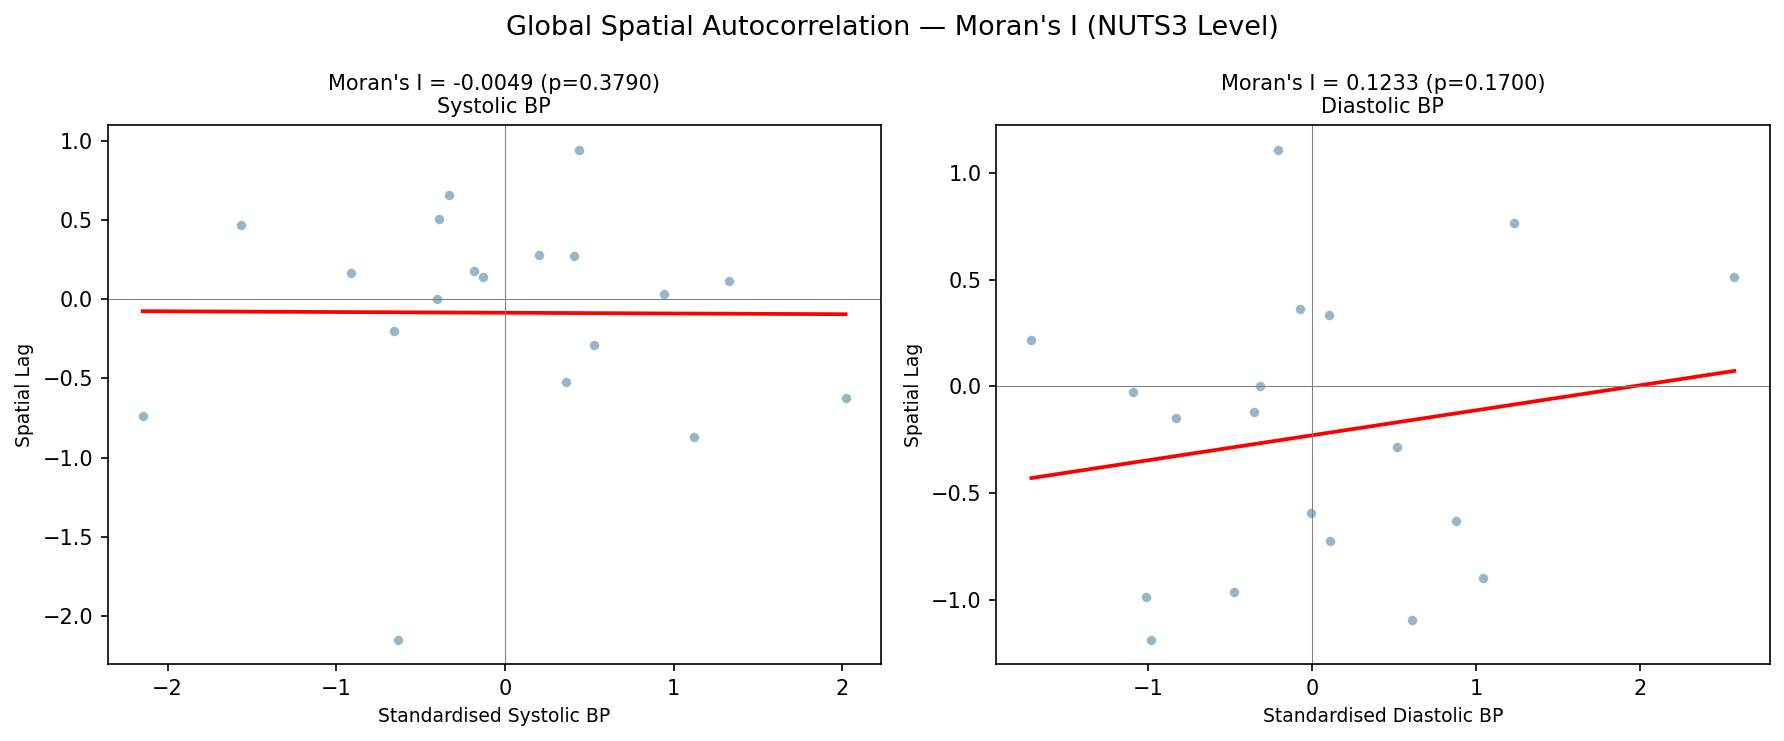
\includegraphics[width=0.85\textwidth]{morans_I_nuts3.png}
\caption{Moran's I analysis at the NUTS3 level.}
\label{fig:morans_nuts3}
\end{figure}

\begin{figure}[H]
\centering
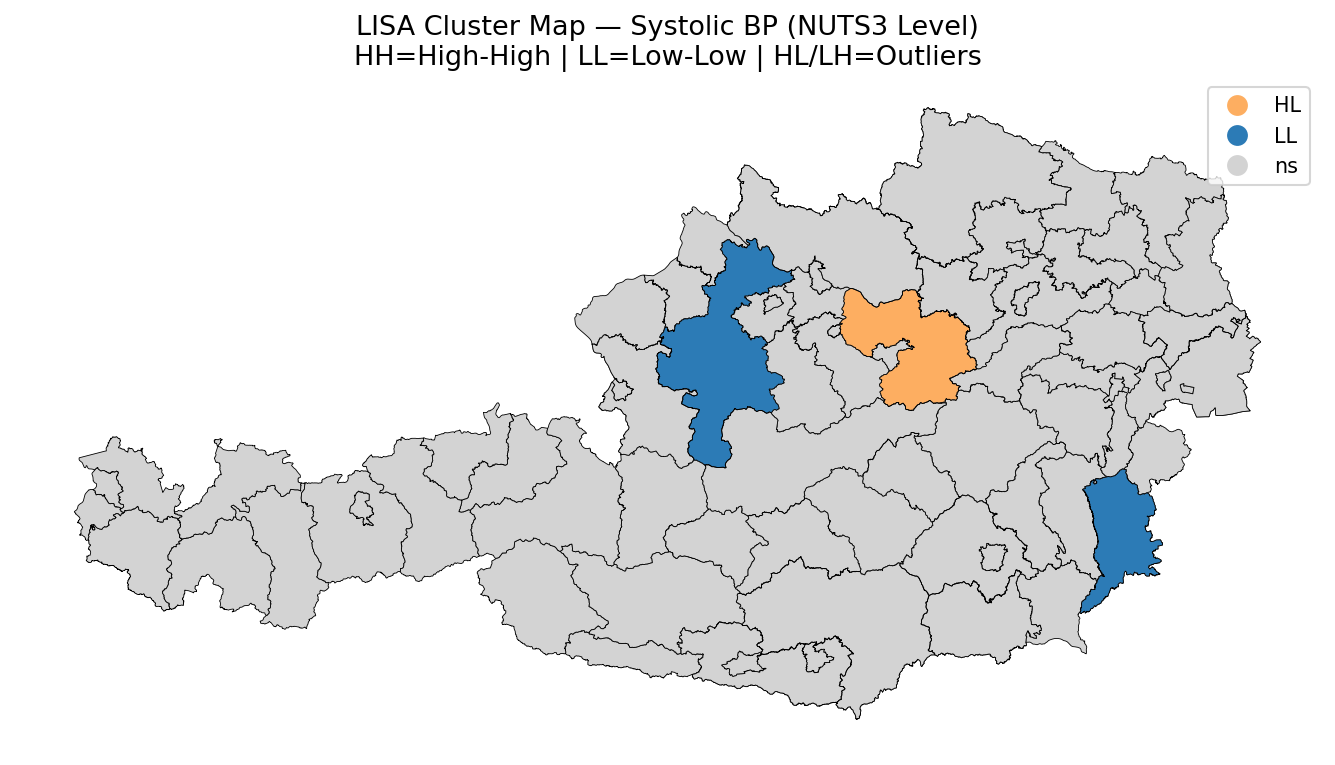
\includegraphics[width=0.70\textwidth]{lisa_clusters_sysbp_nuts3.png}
\caption{LISA cluster map for systolic blood pressure at the NUTS3 level.}
\label{fig:lisa_nuts3}
\end{figure}

Compared with district level results, spatial patterns became substantially weaker. Global spatial autocorrelation was no longer significant, although several local clusters remained visible.

This difference highlights the importance of geographic scale in spatial analysis. Patterns that are clearly visible at the district level become less pronounced when observations are aggregated to larger regions.

\subsection{Socioeconomic Context}

Additional indicators, including disposable income and regional health measures, were examined. Similar to GDP, these variables showed only weak relationships with blood pressure outcomes.

The results suggest that broad regional socioeconomic indicators are insufficient to explain observed spatial variation. More local demographic, environmental, and behavioural factors are likely to play a greater role.

\subsection{Key Findings}

Three conclusions emerge from the spatial analysis.

First, blood pressure exhibits clear geographic structure at the district level, particularly in eastern and southeastern Austria. Second, urban rural classifications explain only a limited proportion of this variation. Third, GDP and disposable income provide little explanatory value despite substantial regional differences in economic performance.

Together, these findings suggest that spatial variation in blood pressure is driven by a combination of local demographic, environmental, and contextual factors rather than broad measures of regional prosperity.
\section{Neighbourhood Effect Analysis}

\subsection{Motivation}

The district and regional analyses presented in the previous section identified clear spatial clustering of blood pressure across Austria. However, geographic patterns may also exist at smaller scales. To investigate whether local context contributes additional information beyond individual characteristics, a neighbourhood effect analysis was conducted using postal code level data.

\subsection{Methodology}

Neighbourhoods were defined using postal code areas. Regions containing fewer than ten observations were excluded, leaving approximately 13,000 observations for analysis.

For each postal code, the mean systolic blood pressure was calculated and assigned to all individuals within that area. This neighbourhood mean was then incorporated into a regression framework as an additional predictor.

The model can be expressed as:

\[
Y = X\beta + N + \varepsilon
\]

where \(Y\) represents individual blood pressure, \(X\beta\) represents individual level predictors, and \(N\) denotes the neighbourhood effect.

To distinguish local and individual variation, blood pressure values were also detrended relative to the neighbourhood mean.

\subsection{Model Comparison}

Two regression models were estimated. The first included only individual level predictors, while the second incorporated neighbourhood mean blood pressure.

\begin{table}[H]
\centering
\caption{Neighbourhood model without neighbourhood predictor.}
\label{tab:neighbourhood_model1}
\begin{tabular}{lc}
\toprule
Variable & Coefficient \\
\midrule
Intercept & 883.42 \\
Year of Birth & -0.39 \\
Smoking & 0.28 \\
Cholesterol Known & 0.34 \\
\bottomrule
\end{tabular}
\end{table}

\begin{table}[H]
\centering
\caption{Neighbourhood model including neighbourhood mean blood pressure.}
\label{tab:neighbourhood_model2}
\begin{tabular}{lc}
\toprule
Variable & Coefficient \\
\midrule
Intercept & 746.76 \\
Year of Birth & -0.37 \\
Smoking & 0.49 \\
Cholesterol Known & 0.55 \\
Neighbourhood Mean BP & 0.83 \\
\bottomrule
\end{tabular}
\end{table}

The neighbourhood coefficient was strongly positive, indicating that individuals living in areas with higher average blood pressure also tended to exhibit higher blood pressure values themselves.

\subsection{Interpretation}

Introducing neighbourhood mean blood pressure changed several coefficient estimates and revealed a substantial neighbourhood effect. The estimated coefficient of 0.83 suggests that local context contributes information beyond the variables available at the individual level.

Several mechanisms may explain this relationship. Neighbourhoods often share socioeconomic characteristics, healthcare accessibility, environmental exposures, and behavioural patterns. The neighbourhood effect may therefore capture influences that are not directly measured elsewhere in the dataset.

Because the analysis is observational, the results should not be interpreted causally. Nevertheless, they provide evidence that local geographic context is associated with blood pressure variation.

\subsection{Relationship to Spatial Clustering}

The neighbourhood analysis complements the district level clustering identified in the previous section. While Moran's I and LISA analyses demonstrated spatial structure across districts, the neighbourhood model indicates that similar patterns remain visible at a much finer geographic scale.

Together, these findings suggest that cardiovascular risk operates across multiple levels of geography, ranging from individual neighbourhoods to larger administrative regions.

\subsection{Limitations}

Several limitations should be considered when interpreting these results. Postal code areas may not correspond perfectly to socially meaningful neighbourhoods, and neighbourhood averages were calculated from the available sample rather than the full population. In addition, neighbourhood mean blood pressure may partly reflect the concentration of high risk individuals rather than contextual influences.

As with the remainder of the study, the cross sectional design prevents causal inference.

\subsection{Key Findings}

The neighbourhood effect analysis identified a strong positive association between local average blood pressure and individual blood pressure. Including neighbourhood information altered several coefficient estimates and strengthened the evidence that geographic context contributes to blood pressure variation.

Combined with the spatial analyses presented earlier, these findings suggest that blood pressure should be viewed not only as an individual level outcome but also as a phenomenon influenced by local environmental and social conditions.


\section{Discussion}

The results provide a consistent picture of blood pressure variation within the Styrian Health Map dataset. Across exploratory analyses, regression models, and machine learning approaches, age emerged as the most influential determinant of blood pressure. Male sex and hypertension treatment status were also associated with higher blood pressure values, whereas smoking, cholesterol awareness, and self reported wellbeing contributed comparatively little explanatory value.

The predictive models achieved only moderate performance. Even after incorporating temporal and environmental variables, a large proportion of blood pressure variation remained unexplained. This finding is not unexpected. Blood pressure is influenced by numerous factors that were unavailable in the dataset, including body mass index, physical activity, dietary habits, medication adherence, stress, and genetic predisposition. The limited predictive performance therefore reflects both the complexity of blood pressure regulation and the constraints of the available data.

The spatial analyses indicate that blood pressure is not distributed randomly across Austria. Significant clustering was observed at the district level, particularly in eastern and southeastern regions. At the same time, broad socioeconomic indicators such as GDP and disposable income showed only weak associations with blood pressure outcomes. This suggests that local contextual factors may be more relevant than regional economic conditions alone.

One of the most notable findings is the neighbourhood effect identified in the final analysis. Individuals living in areas with higher average blood pressure were also more likely to exhibit elevated blood pressure themselves, even after accounting for individual characteristics. Together with the district level clustering results, this finding suggests that cardiovascular risk operates across multiple geographic scales.

The study has several strengths. The dataset contains a large number of observations, allowing multiple analytical approaches to be applied within a single framework. The combination of statistical modelling, machine learning, and spatial analysis provides a broader perspective than any single method alone.

Several limitations should also be acknowledged. The cross sectional design prevents causal inference, and important clinical and lifestyle variables were unavailable. In addition, changes in measurement devices during data collection may have introduced additional variability. These limitations should be considered when interpreting the results.

Despite these constraints, the findings demonstrate that blood pressure variation is shaped by both individual characteristics and geographic context. The consistency of results across multiple analytical approaches increases confidence in the robustness of the main conclusions.


\section{Conclusion}

This study investigated blood pressure variation using data from the Styrian Health Map project. By combining exploratory analysis, linear regression, machine learning, classification techniques, and spatial methods, the study examined demographic, clinical, environmental, and geographic influences on blood pressure.

Several conclusions emerge from the analysis. Age was the most consistent predictor across all modelling approaches, while male sex and hypertension treatment status were also strongly associated with elevated blood pressure. Random Forest models demonstrated that blood pressure can be predicted to a limited extent using the available variables, although a large proportion of variation remained unexplained. Classification models were more successful in identifying elevated blood pressure categories than predicting exact blood pressure values.

The spatial analyses revealed meaningful geographic structure, particularly at the district level. Regional economic indicators showed only weak associations with blood pressure outcomes, whereas neighbourhood level analyses suggested that local context contributes additional explanatory information beyond individual characteristics.

Overall, the findings indicate that blood pressure variation is influenced by a combination of individual characteristics and geographic context. While the available variables were sufficient to identify several important patterns, they were not sufficient to fully explain or accurately predict blood pressure outcomes. Future studies incorporating additional clinical, behavioural, and socioeconomic information may provide a more complete understanding of the mechanisms underlying blood pressure variation.


\end{document}